\documentclass{article}

\usepackage[utf8]{inputenc}

\usepackage{amsmath, bm}
\usepackage{graphicx}
\usepackage{amssymb}
\usepackage{float}
\usepackage{caption}
\usepackage{subcaption}
% set font size to 11pt
% set margin
\usepackage[margin=0.5in]{geometry}

\setlength{\parskip}{\baselineskip}%
\setlength{\parindent}{0pt}%

\begin{document}

% insert pdf cover page here

\title{Lab report: 3A3 Supersonic Nozzle}
\author{lwp26}
\date{December 2023}
\maketitle

\begin{abstract}
    \centering
    % write a brief summary of the experiment and the results
    Uhm this is the abstract which will be written at the end!
\end{abstract}

\section{Introduction}

\subsection{Purpose}
% explaining the significance of supersonic nozzles to wind tunnels and other applications.
% The converging-diverging nozzle is a device that can accelerate a fluid to supersonic speeds, and is used in both aircraft and wind tunnels.
The converging-diverging nozzle is a device that can accelerate a fluid to supersonic speeds, and is used in many engineering applications, such as the design of supersonic wind tunnels, supersonic aircraft and rocket engines.
Supersonic nozzles are essential components in wind tunnels designed to simulate high-speed conditions that objects experience in flight.
By accelerating airflow to supersonic speeds, these nozzles enable researchers to recreate the aerodynamic forces and flow patterns that occur at high speeds.
This is also done at a smaller scale through dimensional analysis which significantly reduces the cost of testing.

% explain the purpose of the experiment

\subsection{Objectives}
% list the objectives of the experiment

\begin{itemize}
    \item To study the static pressure distribution in a converging-diverging nozzle for 4 different pressure ratios across the nozzle.
    \item To appreciate the validity and limitations of one-dimensional, adiabatic, inviscid theory for calculating mass flow rate from the pressure drop across an oriface plate.
    \item To obtain 10 marks for the full technical report.
\end{itemize}

\section{Theory}
% Introduce the essential relationships necessary to explain your results in the later section. Refer to these
% equations in the later sections. (You need not derive these relationships but you should explain in words why
% they are needed and reference their source).

\subsection{Mass flow rate though oriface plate}

The following assumptions are made to derive a relationship for the mass flow rate through an orifice plate.
\begin{itemize}
    \item The flow into the orifice is inviscid,
    \item The flow is slow enough to be treated as incompressible with density equal to that in the atmosphere upstream of the orifice (where the velocity is negligible),
    \item The velocity is uniform across the plane of the orifice,
    \item The pressure difference between the orifice plane and the upstream atmosphere is that measured on the water manometer
\end{itemize} 

With both the invicid and incompressible assumptions, the ideal flow rate through the orifice can be calculated using the pressure difference between the orifice plane and the upstream atmosphere is that measured on the
water manometer. By applying the Bernoulli equation from the upstream atmosphere (1) to the orifice plane (2),

\begin{equation}
    p_1 = p_2 + \frac{1}{2} \rho_a v_2^2
\end{equation}

Where $A$ and $v_2$ are the cross-sectional area, and velocity at the orifice. The pressure in the centre of the oriface is taken to be equal to the value measured at the wall, due to the assumption that the velocity is uniform across the oriface plane.
The theoretical mass flow rate through the orifice is then given by the following equation.
\begin{equation}
    \dot{m}_{ideal} = \rho_a A v_2 = \rho_a \left( \frac{\pi D^2}{4}\right) \sqrt{\frac{2(p_1-p_2)}{\rho_a}} \;\;\;\;\;\; \text{where} \;\;\;\;\;\ p_2 - p_1 = \rho_w g \Delta h
\end{equation}
Where $\rho_a$ is the density of air and $\rho_w$ is the density of water used for the manometer.

However, the actual flow rate through the orifice differs from the theoretical value as our assumptions are not valid.
The first assumption is not valid as there is significant viscous dissipation before the orifice. However, these losses are accounted for by a discharge coefficient $C_d$, which is defined as the ratio of actual discharge to the ideal discharge.
The value of $C_d$ is constant at the high Reynolds numbers considered in this report.
To analyse the validity of the second assumption, consider the case of maximum flow, when the nozzle is choked upstream of the orifice, then its non-dimensional mass flow rate is given by the following equation.
\begin{equation}
    \frac{\dot{m}\sqrt{c_pT_0}}{p_0A^*} = 1.281
\end{equation}
From this, the non-dimensional mass flow rate at the orifice can be calculated using the area ratio of the orifice to the nozzle throat.
The area of the throat is approximately $24\text{mm}^2$, and so the non-dimensional mass flow rate at the orifice is $0.1282$.
At this point, the corresponding density ratio $\rho/\rho_0 = 0.9997 \approx 1$. This means that the density change is negligible and can be ignored.

The third assumption that the velocity is uniform is also poor, and is accounted for by the discharge coefficient $C_d$.
This difference is characterised by the discharge coefficient $C_d$ which is defined as the ratio of the actual flow rate to the theoretical flow rate.
\begin{equation}
    \dot{m}_{actual} = C_d \dot{m}_{ideal}
\end{equation}

The discharge coefficient of the orifice is effectively constant over the range of high reynolds numbers considered in this experiment.
This was shown by Graham and Webster \cite{Graham_K_Webster:2019} in figure \ref{fig:const_Cd_Re}.

\subsection{Pressure tappings}

The static pressure at a specific pressure tapping along the nozzle is given by the following equation.
\begin{equation}
    p = p_0 - \rho_{Hg} g \Delta h
\end{equation}
Where $\rho_{Hg}$ is the density of mercury and $\Delta h$ is the height difference of mercury between the specific pressure tapping and atmospheric tapping.

The static pressure ratio across the nozzle is given by the following equation.
\begin{equation}
    \frac{p}{p_0} = 1 - \frac{\rho_{Hg} g \Delta h}{p_0}
\end{equation}

\subsection{Mach number}
For isentropic flow and a given static pressure ratio across the nozzle, the Mach number can be found by rearanging the following equation.
\begin{equation}
    \frac{p}{p_0} = \left( 1 + \frac{\gamma - 1}{2}M^2\right) ^ {-\frac{\gamma}{\gamma-1}} \implies M = \sqrt{\frac{2}{\gamma-1} \left( \left( \frac{p}{p_0}\right) ^ {-\frac{\gamma-1}{\gamma}} - 1\right)}
\end{equation}
And then the nozzil area ratio can be found using the following equation from the Mach number found above.
\begin{equation}
    \frac{A}{A^*} = \frac{1}{M} \left( \frac{2}{\gamma+1} \left( 1 + \frac{\gamma-1}{2}M^2\right) \right) ^ {\frac{\gamma+1}{2(\gamma-1)}}
\end{equation}
For case 3 there is a drop in stagnation pressure accross the shock wave and so after the shock, the stagnation pressure is no longer the atmospheric pressure.
For the region behind the shock, this is accounted for by dividing the original static pressure ratio by the ratio of stagnation pressures accross the shock wave.
\begin{equation}
    \frac{p}{p_{0s}} = \frac{p/p_0}{p_{0s}/p_0}
\end{equation}
The stagnant pressure before and after the shock is given by $p_0$ and $p_{0s}$ respectively.
The stagnation pressure ratio accross the shock wave is given in the databook \cite{data_book}.
\begin{equation}
    \frac{p_{0s}}{p_0} = \left( \frac{\frac{\gamma+1}{2}M^2}{1 + \frac{\gamma-1}{2}M^2}\right) ^ \frac{\gamma}{\gamma-1} \left( \frac{2\gamma}{\gamma+1} M^2 - \frac{\gamma-1}{\gamma+1}\right) ^ \frac{1}{1 - \gamma}
\end{equation}
Where $M$ is the Mach number before the shock wave.

\subsection{Schlieren visualisation technique}

WRITE THIS SECTION CORRECTLY
Mazumdar et al. \cite{Mazumdar_Amrita:2013} described the Schlieren visualisation technique as a method of visualising the density gradient of a fluid.


\iffalse
\begin{figure}[H]
    \centering
    \begin{subfigure}[t]{0.7\textwidth}
        \centering
        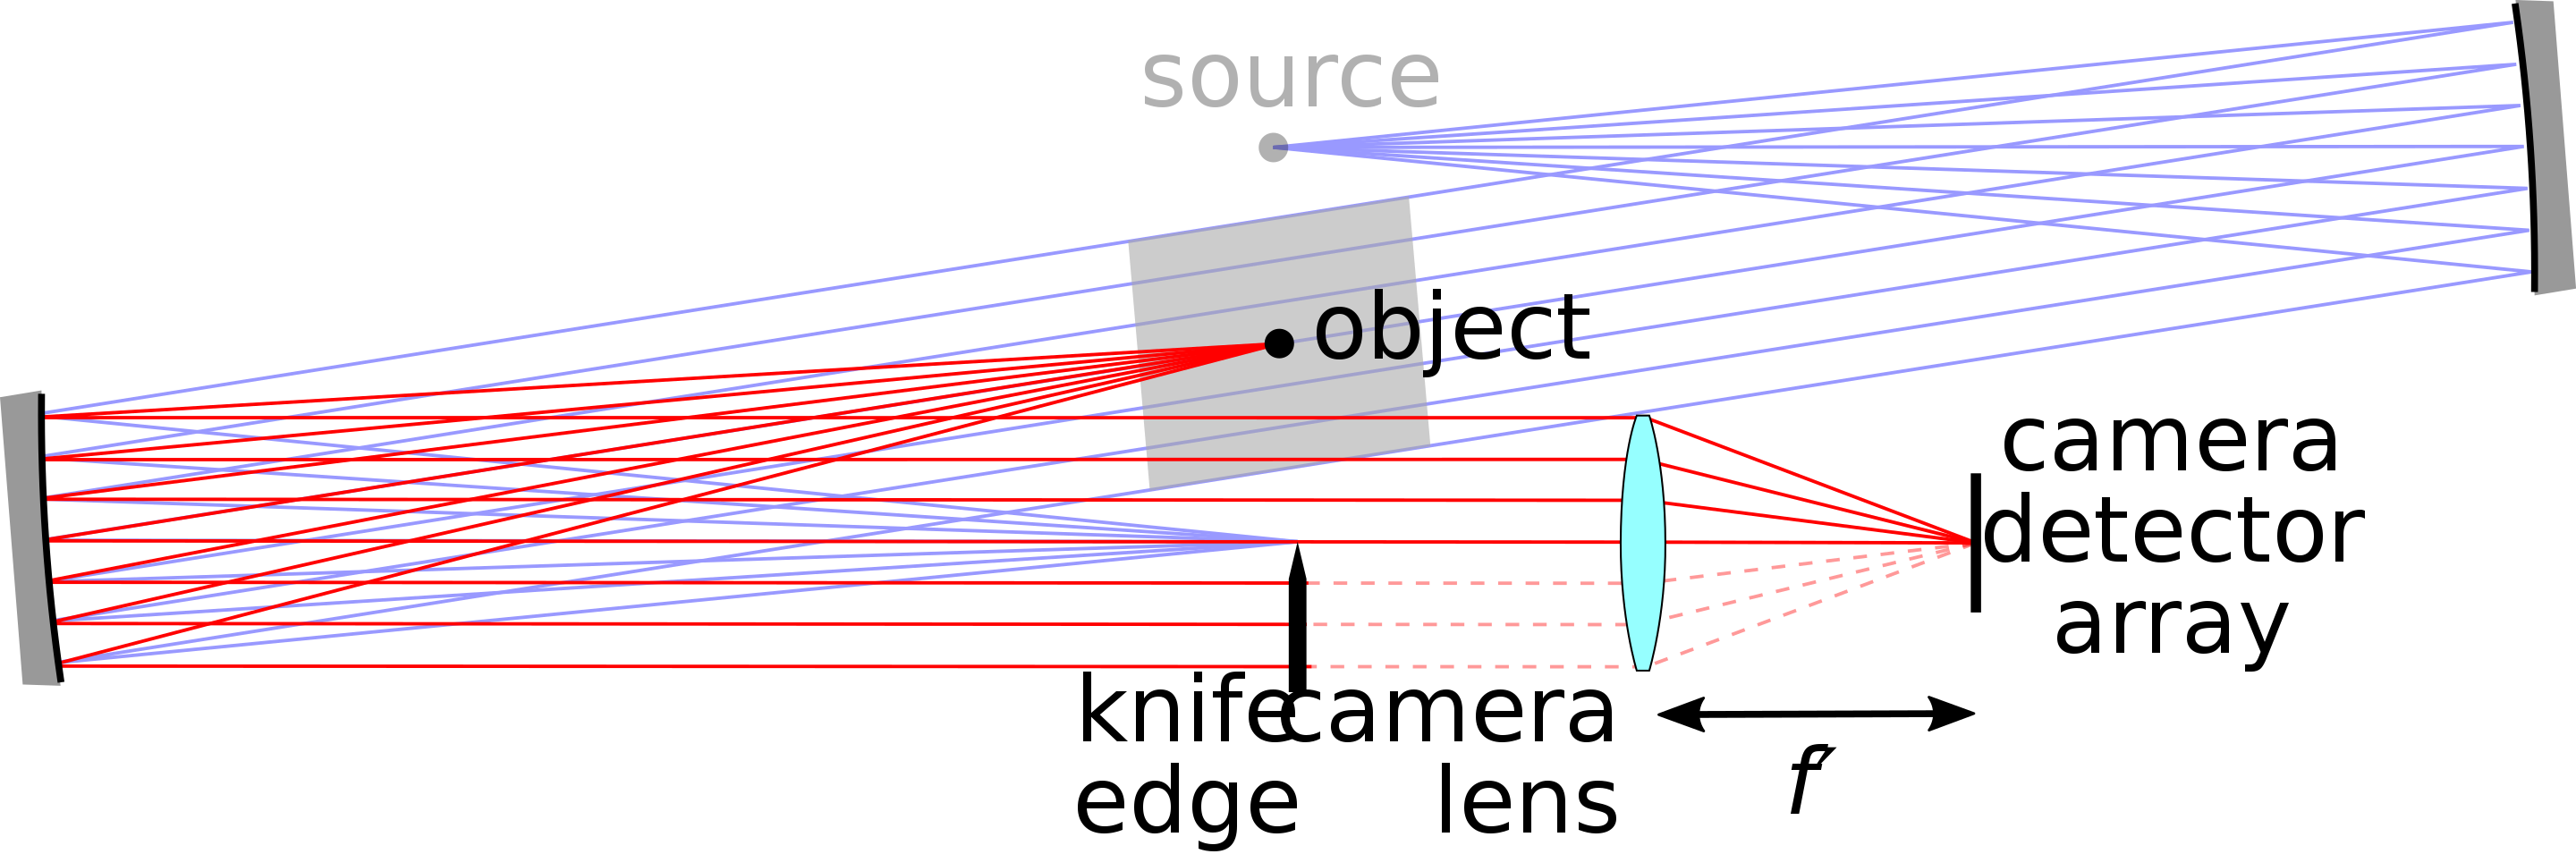
\includegraphics[width=1\textwidth]{Double_mirror_schlieren_layout.png}
        \caption{heading}
        \label{fig:mirror_setup}
    \end{subfigure}
    ~
    \begin{subfigure}[t]{0.28\textwidth}
        \centering
        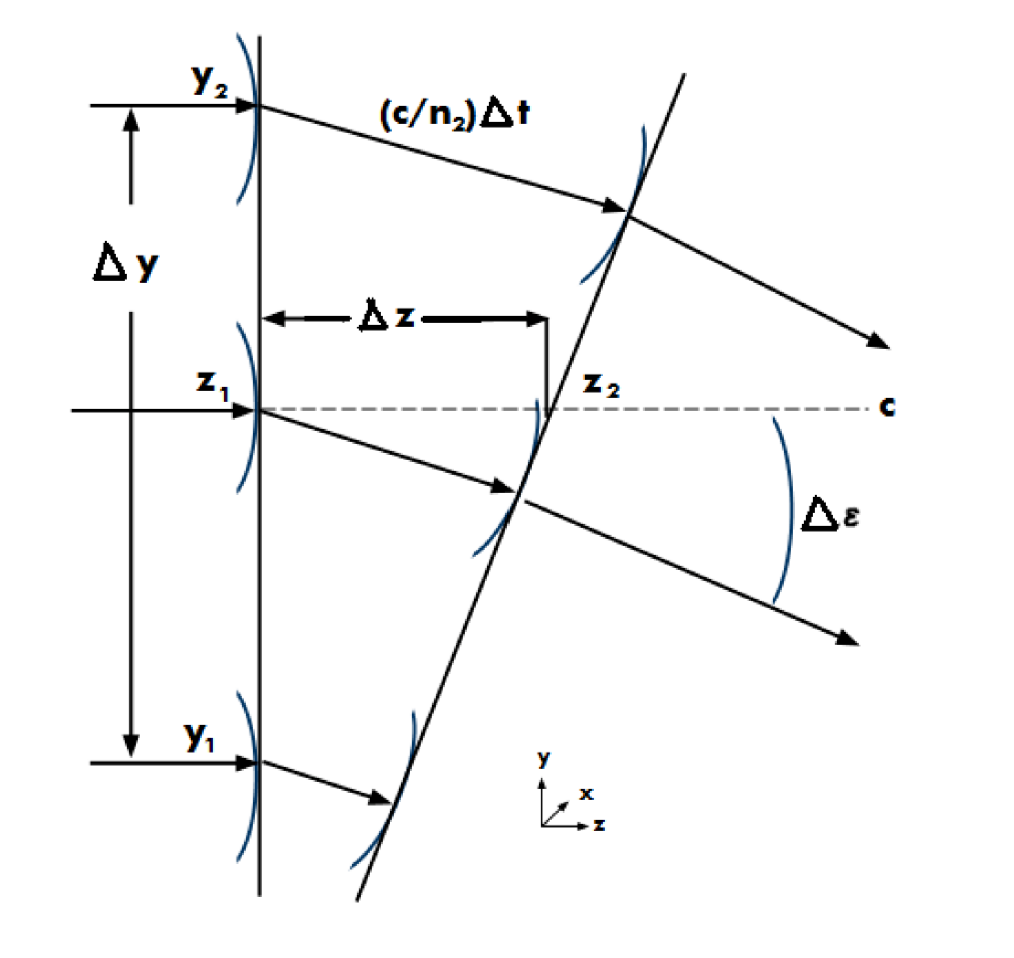
\includegraphics[width=1\textwidth]{Mazumdar_Amrita_shlierien_refraction.png}
        \caption{Top down view of light ray deflection by refractive index gradient $dn/dy$ \cite{Mazumdar_Amrita:2013}.}
        \label{fig:refraction_diagram}
    \end{subfigure}
    \caption{Shlieren visualisation technique \cite{Mazumdar_Amrita:2013}.}
\end{figure}
\fi

\begin{figure}[H]
    \centering
    \begin{subfigure}[t]{0.8\textwidth}
        \centering
        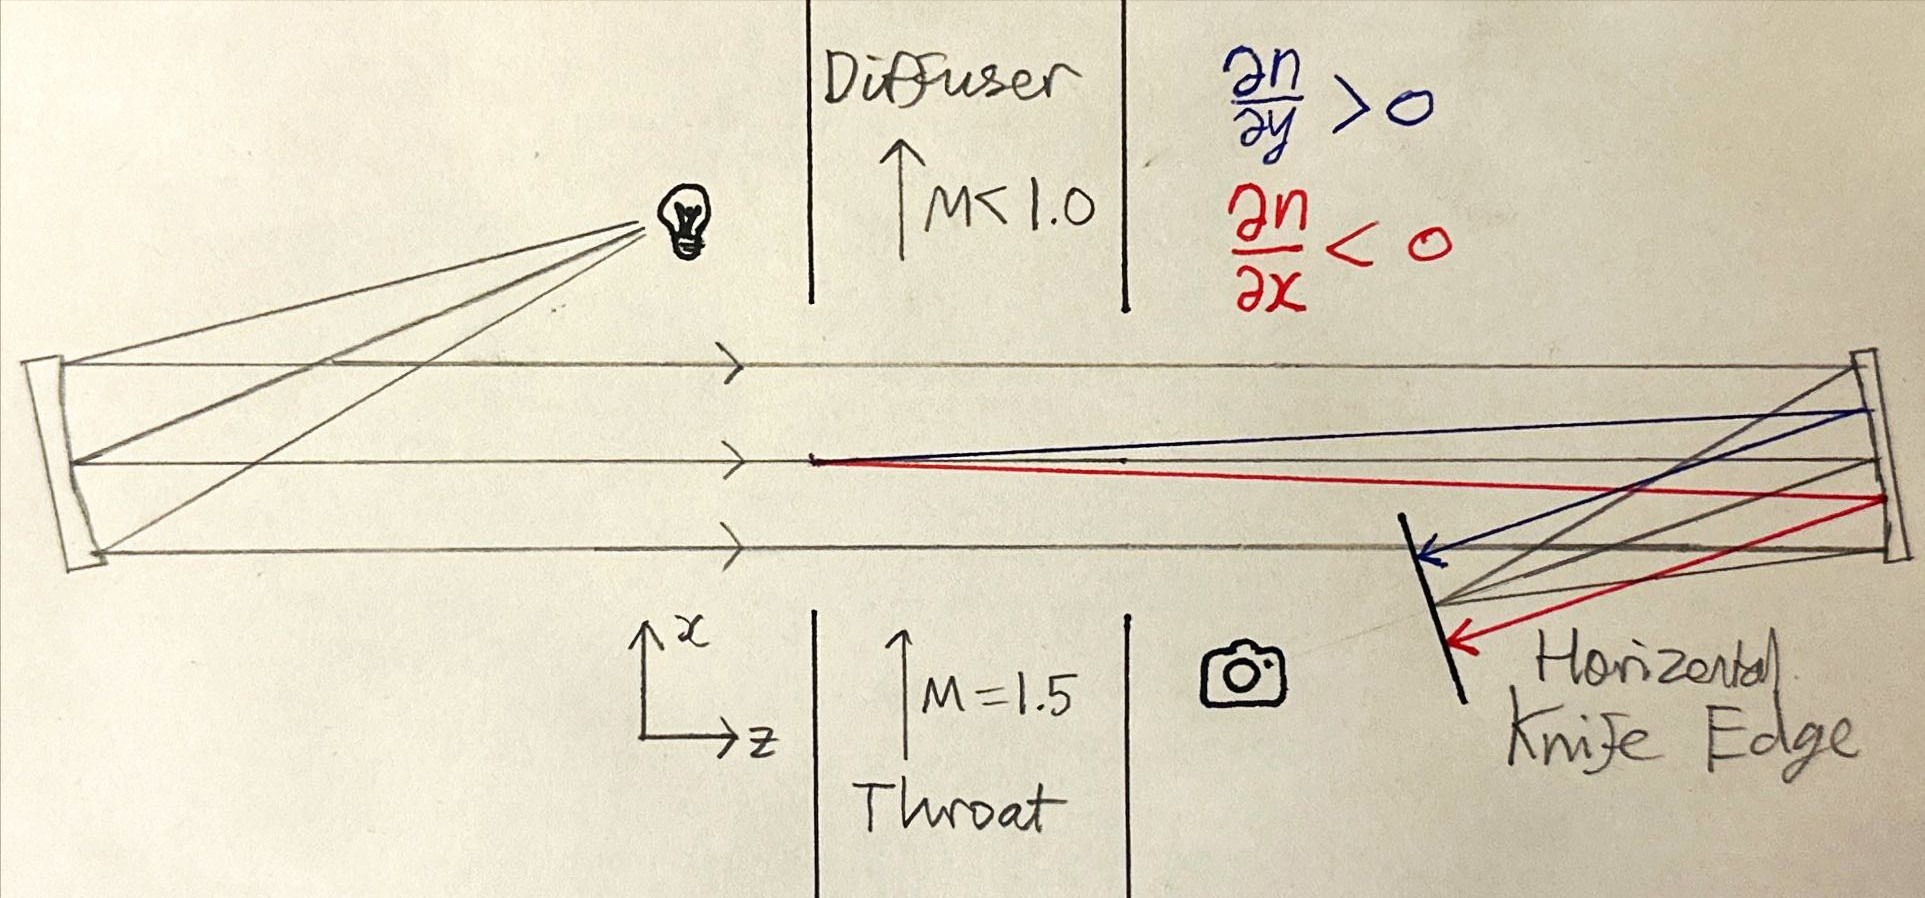
\includegraphics[width=1\textwidth]{xz_shlierian.jpg}
        \caption{Sketch of light rays passing through refractive index gradient in xz plane.}
        \label{fig:xz_shlierian}
    \end{subfigure}
    ~
    \begin{subfigure}[t]{0.8\textwidth}
        \centering
        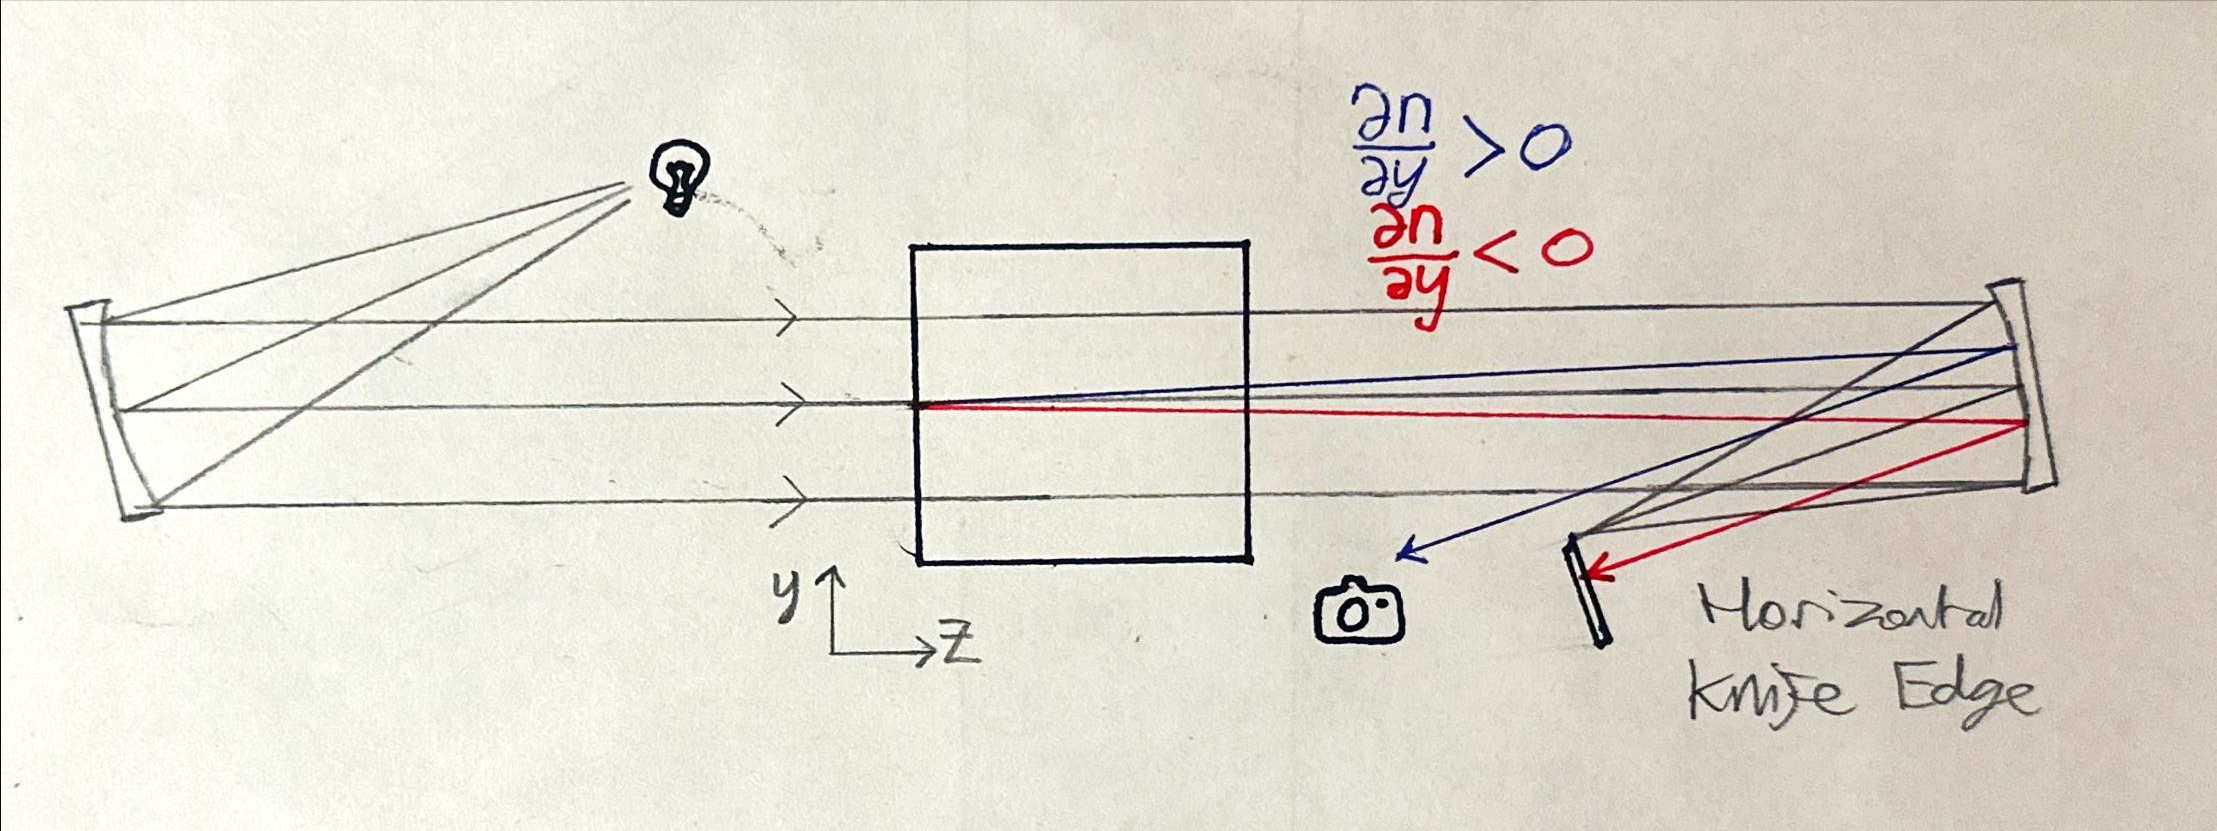
\includegraphics[width=1\textwidth]{yz_shlierian.jpg}
        \caption{Sketch of light rays passing through refractive index gradient in yz plane.}
        \label{fig:yz_shlierian}
    \end{subfigure}
    \caption{Shlieren visualisation technique \cite{Mazumdar_Amrita:2013}.}
\end{figure}

\begin{equation}
    \epsilon_y = \frac{1}{n}\int \frac{\partial n}{\partial y} dz
    \label{eqn:refractive_index_gradient}
\end{equation}
For a small angle approximation 

Equation 1 indicates it is not the refractive index n causing ray deflection, but the gradient $\partial n / \partial y$ of this refractive index.
Additionally, Eqns. 1 and 2 show light ray deflections bend towards regions of higher refractive index.

For this normal shock wave the density can be considered as a step function of y.
This is because the thickness of the shock is on the order of a few molecular-mean-free paths \cite{babinsky_delery:2011}.
Figure \ref{fig:refractive_index_vs_density} shows the relationship between the refractive index and density of air at specified conditions.
The refractive index can be approximated as a linear function of the density and so the gradient of the refractive index step function is now a dirac delta function.

When this is integrated over the thickness of the shock, it gives a angle of deflection of the light ray which is proportional to the density gradient.
This means that regions of 




\section{Method}
\subsection{Part 1}
\subsubsection{Apparatus}

\begin{figure}[H]
    \centering
    \begin{subfigure}{0.8\textwidth}
        \centering
        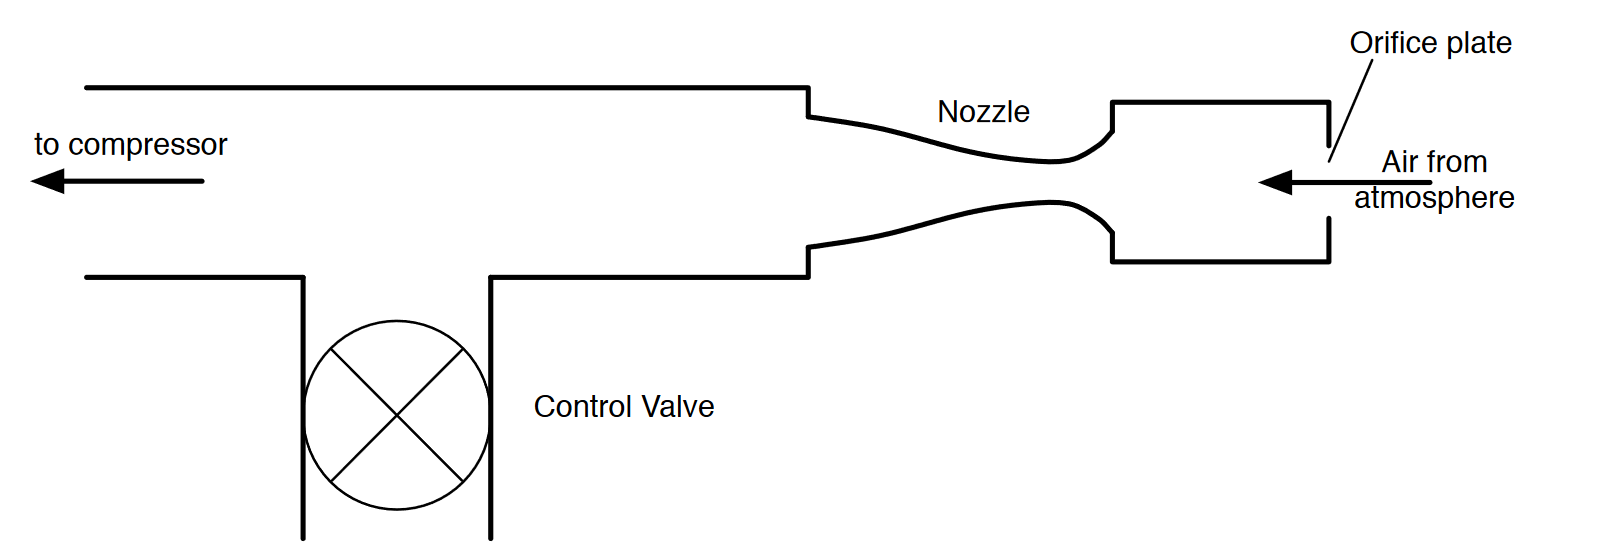
\includegraphics[width=0.6\textwidth]{flow_layout.png}
        \caption{Flow path diagram}
        \label{fig:flow_layout}
    \end{subfigure}
    ~
    \begin{subfigure}{0.8\textwidth}
        \centering
        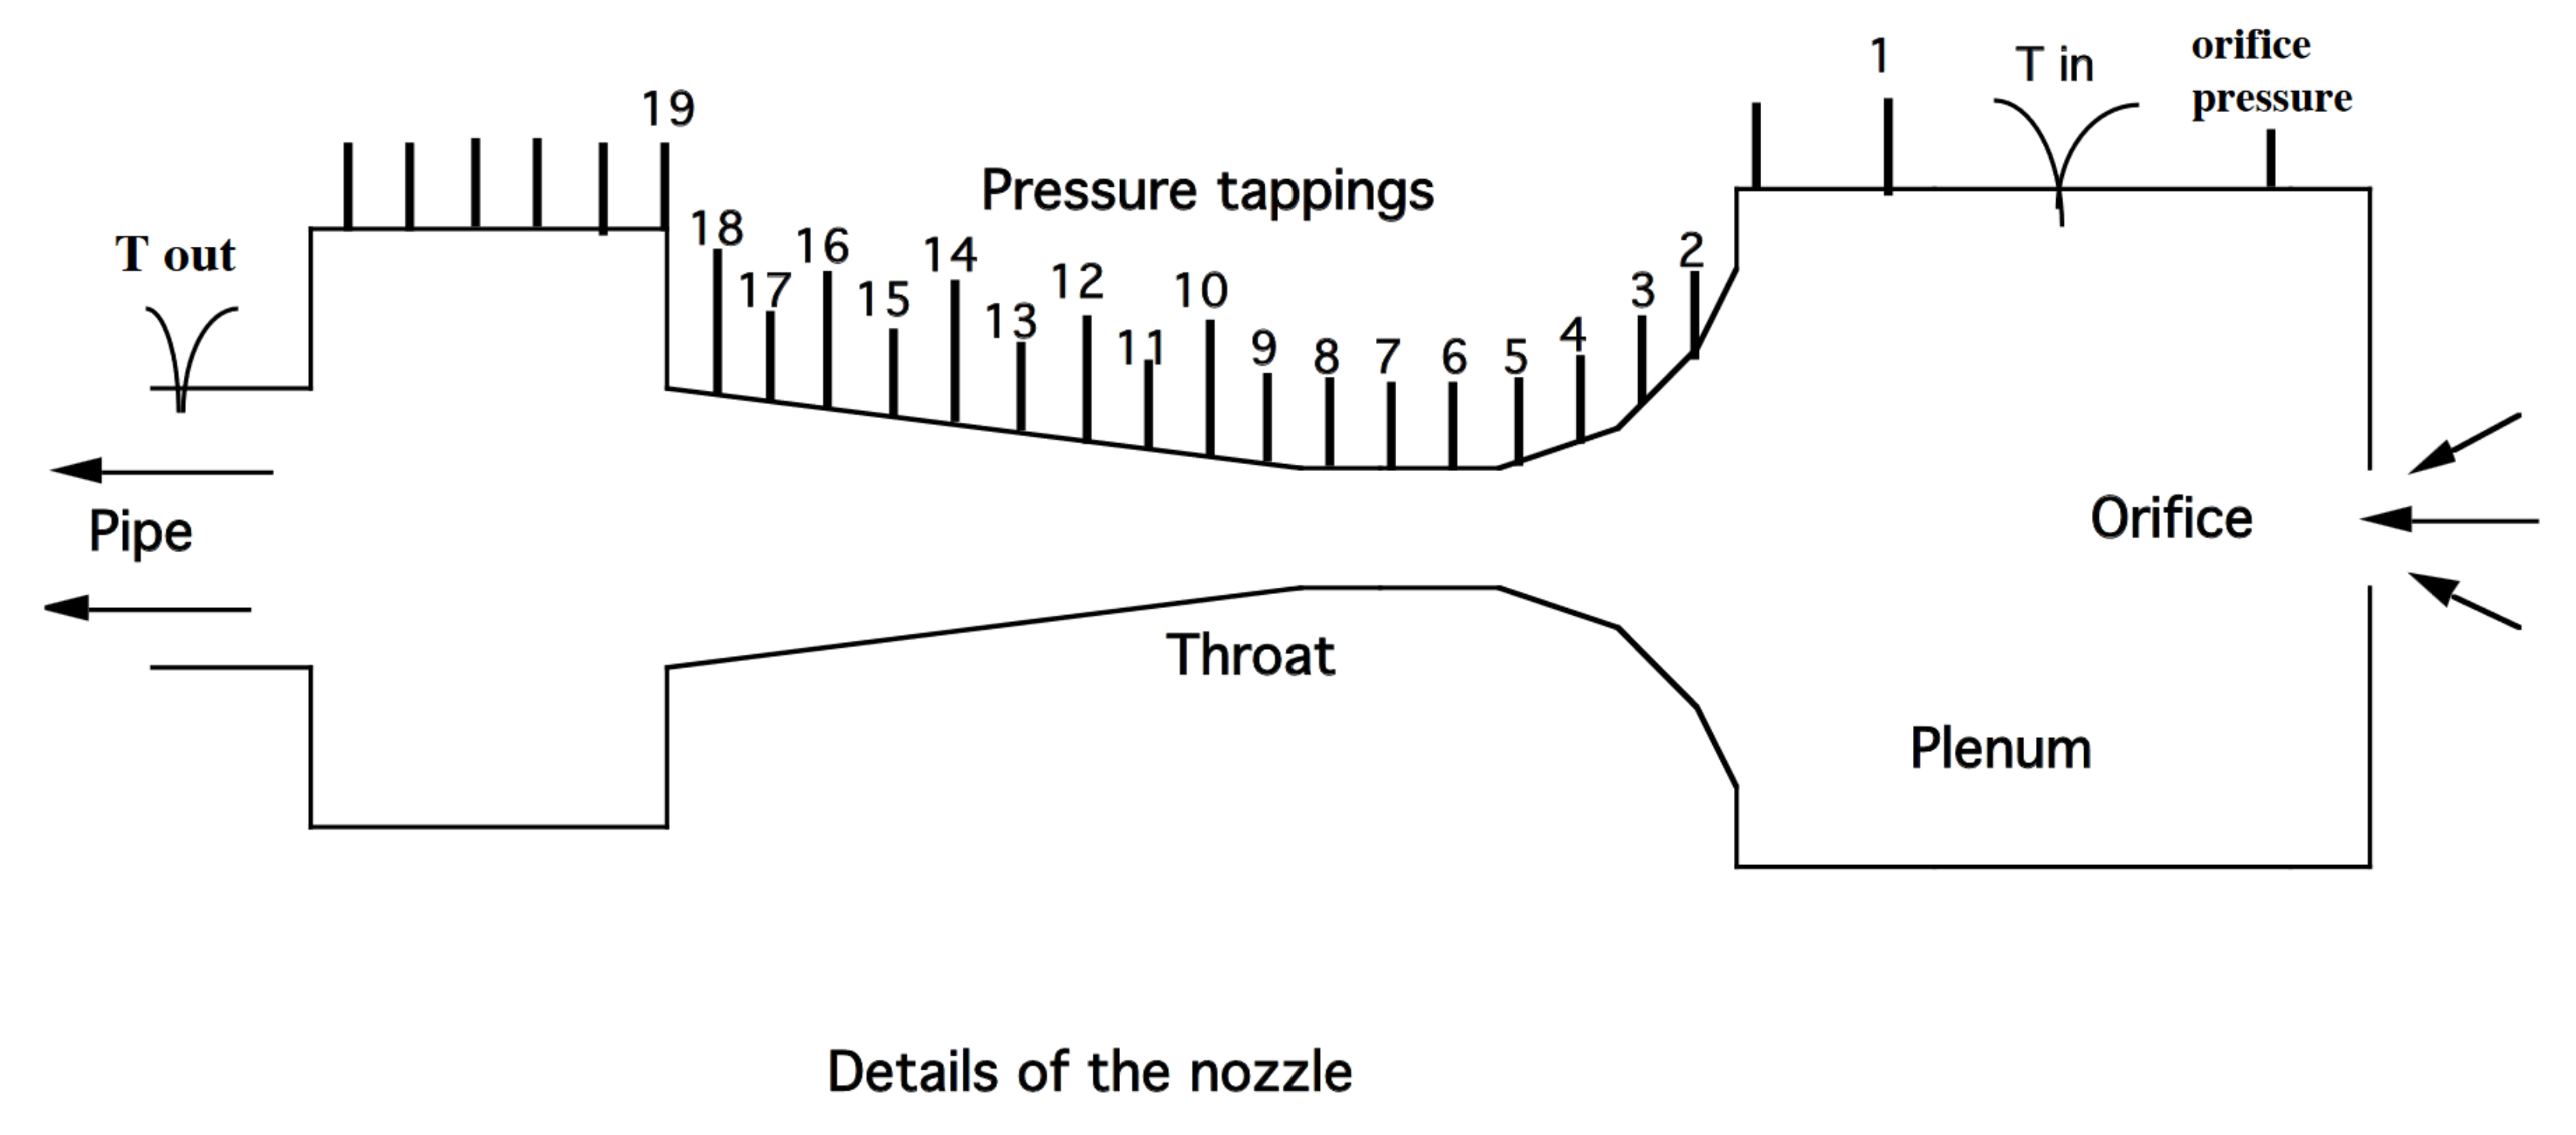
\includegraphics[width=0.6\textwidth]{../Supersonic_Nozzle/small_nozzle_layout.png}
        \caption{Nozzle layout diagram}
        \label{fig:nozzle_layout}
    \end{subfigure}
    \caption{Experiment apparatus \cite{lab_manual}.}
\end{figure}

The apparatus used in this experiment is shown in figure \ref{fig:flow_layout}.
A control valve is used to control the pressure of the air downstream of the nozzle. By closing the valve, the pressure downstream of the nozzle decreases, and so pressure ratio across the nozzle increases.
The pressure at each tapping along the nozzle is measured using a series of 19 vertical mercury manometers.
The pressure difference accross the oriface is a smaller pressure drop and so is measured using a vertical water manometer.

\subsubsection{Procedure}

Values for temperature and atmospheric pressure were taken from a gauge and mercury manometer in the lab.
A preliminary experiment was conducted to determine the pressure ratio at which the nozzle is choked.
This was done by closing the valve and increasing the pressure ratio across the nozzle until there was no change in the oriface plate manometer readings.
This approximate height difference of the manometer at the choking point was then recorded.

Then the first operating point was reached by setting the height difference of the manometer to $70\%$ of that of the choking point.
This took a few iterations of adjusting the control valve, waiting for the water manometer to settle and reading both manometers to find the height difference.
After a stable setpoint is reached, the measured oriface manometer height readings were recorded. 
Then all 19 manometer wall tappings and the atmospheric were recorded.
It was noted that tapping 8 had the lowest pressure and so was taken to be the throat of the nozzle.

The second operating point was then reached by setting the height difference of the manometer that of the choking point.
Recording of oriface manometer height readings and all 19 manometer wall tappings and the atmospheric were repeated.

The third operating point is when a shock forms in the diverging part of the nozzle. The valve was closed until the manometer height at the throat, at tapping 8, was equal to the height at tapping 16.
This was because the location of the shock wave was approximated to be where the flow dropped below Mach 1.
This was found to be particularly difficult as the manometer height at tapping 16 was very sensitive to changes in the valve position.
A sufficient setpoint was found and the oriface plate manometer height readings were recorded.
Then again all 19 manometer wall tappings and the atmospheric were recorded.

The fourth and final run was conducted by closing the valve entirely so there was maximum pressure ratio across the nozzle.
Then the oriface plate manometer heights, all 19 manometer wall tappings and the atmospheric were recorded.

\subsection{Uncertainty}

Naturally, there are sources of uncertainty in all measurements taken and so it is important for all calculations to include an estimate of the uncertainty in the final result.
The uncertainty equations are derived from the equation for the quantity being calculated.
To simplify the analysis the uncertainty in the discharge coefficient and densities of water and mercury are assumed to be negligible.
The uncertainty in pressure ratio is calculated using the following equation.
\begin{equation}
    u\left( \frac{p}{p_0} \right) = u(\rho_{Hg}) + u(\Delta h) + u(p_0)
\end{equation}
The uncertainty in mass flow rate is calculated using the following equation.
\begin{equation}
    u(\dot{m}) = u(C_d) + 2u(D) + \frac{1}{2}u(\rho_a) + \frac{1}{2}u(\Delta h)
\end{equation}

% dM2 = - 2 / g * rp ** (-((g-1)/g) - 1)
The uncertainty in Mach number is calculated using the following equation.
\begin{equation}
    u(M) = u\left( \frac{p}{p_0} \right) \frac{d M ( p/p_0 ) }{d (p/p_0)} = u\left(\frac{p}{p_0}\right) \times - \frac{2}{\gamma}  \left( \frac{p}{p_0} \right) ^ {\frac{1}{\gamma}}
\end{equation}
Further uncertainty analysis in the area ratio and stagnant pressure ratio accross the shock wave is covered in the appendix.
Uncertainty analysis is not conducted for the location of the shock wave as this is already a very rough approximation due to boundary layer effects.

\subsection{Part 2}
\subsubsection{Procedure}
\subsubsection{Apparatus}

\section{Results}

\begin{center}
    \begin{tabular}{|c|c|c|c|c|}
    \hline 
    Case & Throat Mach No.  & Exit Mach No. & Mass flow rate & Calculated Throat Area\\
     & (-) & (-) & $\times 10^{-3}$ kg/s & $mm^2$ \\
    \hline 
    1 & $0.602\pm 0.003$ & $0.491\pm 0.005$ & $ 4.25\pm 0.42  $ & \\
    2 & $1.063\pm 0.017$ & $0.715\pm 0.007$ & $ 4.96\pm 0.36  $ & \\
    3 & $1.063\pm 0.017$ & $0.800\pm 0.036$ & $ 4.96\pm 0.36 $ & \\
    4 & $1.068\pm 0.017$ & $1.420\pm 0.064$ & $ 4.96\pm 0.36 $ & \\
    \hline
    \end{tabular}
    \captionof{table}{Exit and throat Mach numbers for each case.}
    \label{tab:1}
\end{center}

\begin{figure}[H]
    \centering
    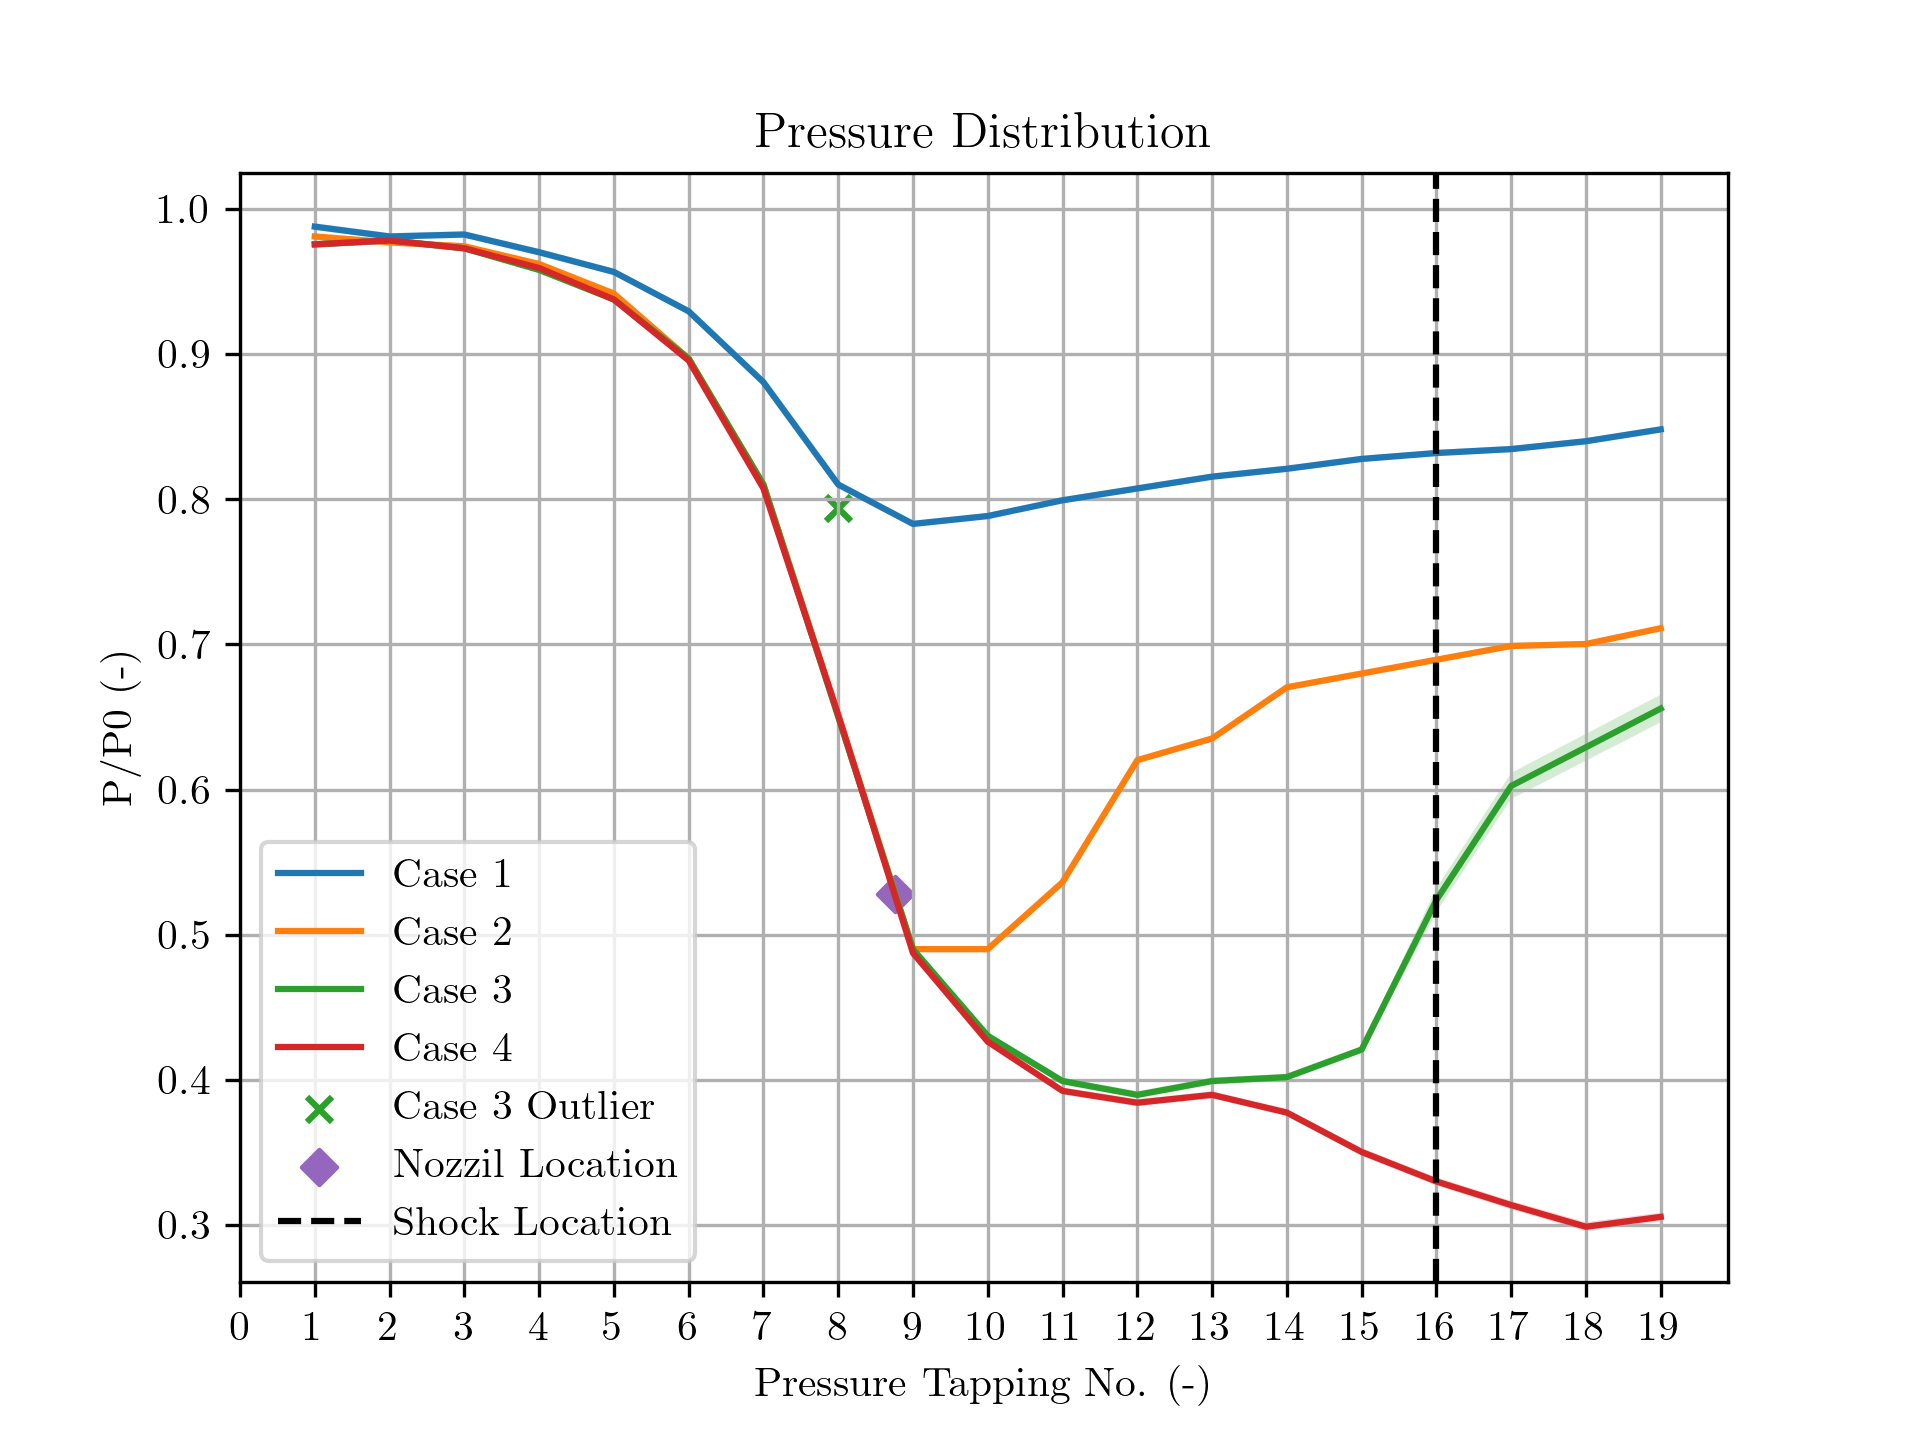
\includegraphics[width=0.98\textwidth]{../Supersonic_Nozzle/pressure_ratio_distribution_corrected.png}
    \caption{Static pressure ratio distribution along the nozzle.}
    \label{fig:pressure_distribution}
\end{figure}

\begin{figure}[H]
    \centering
    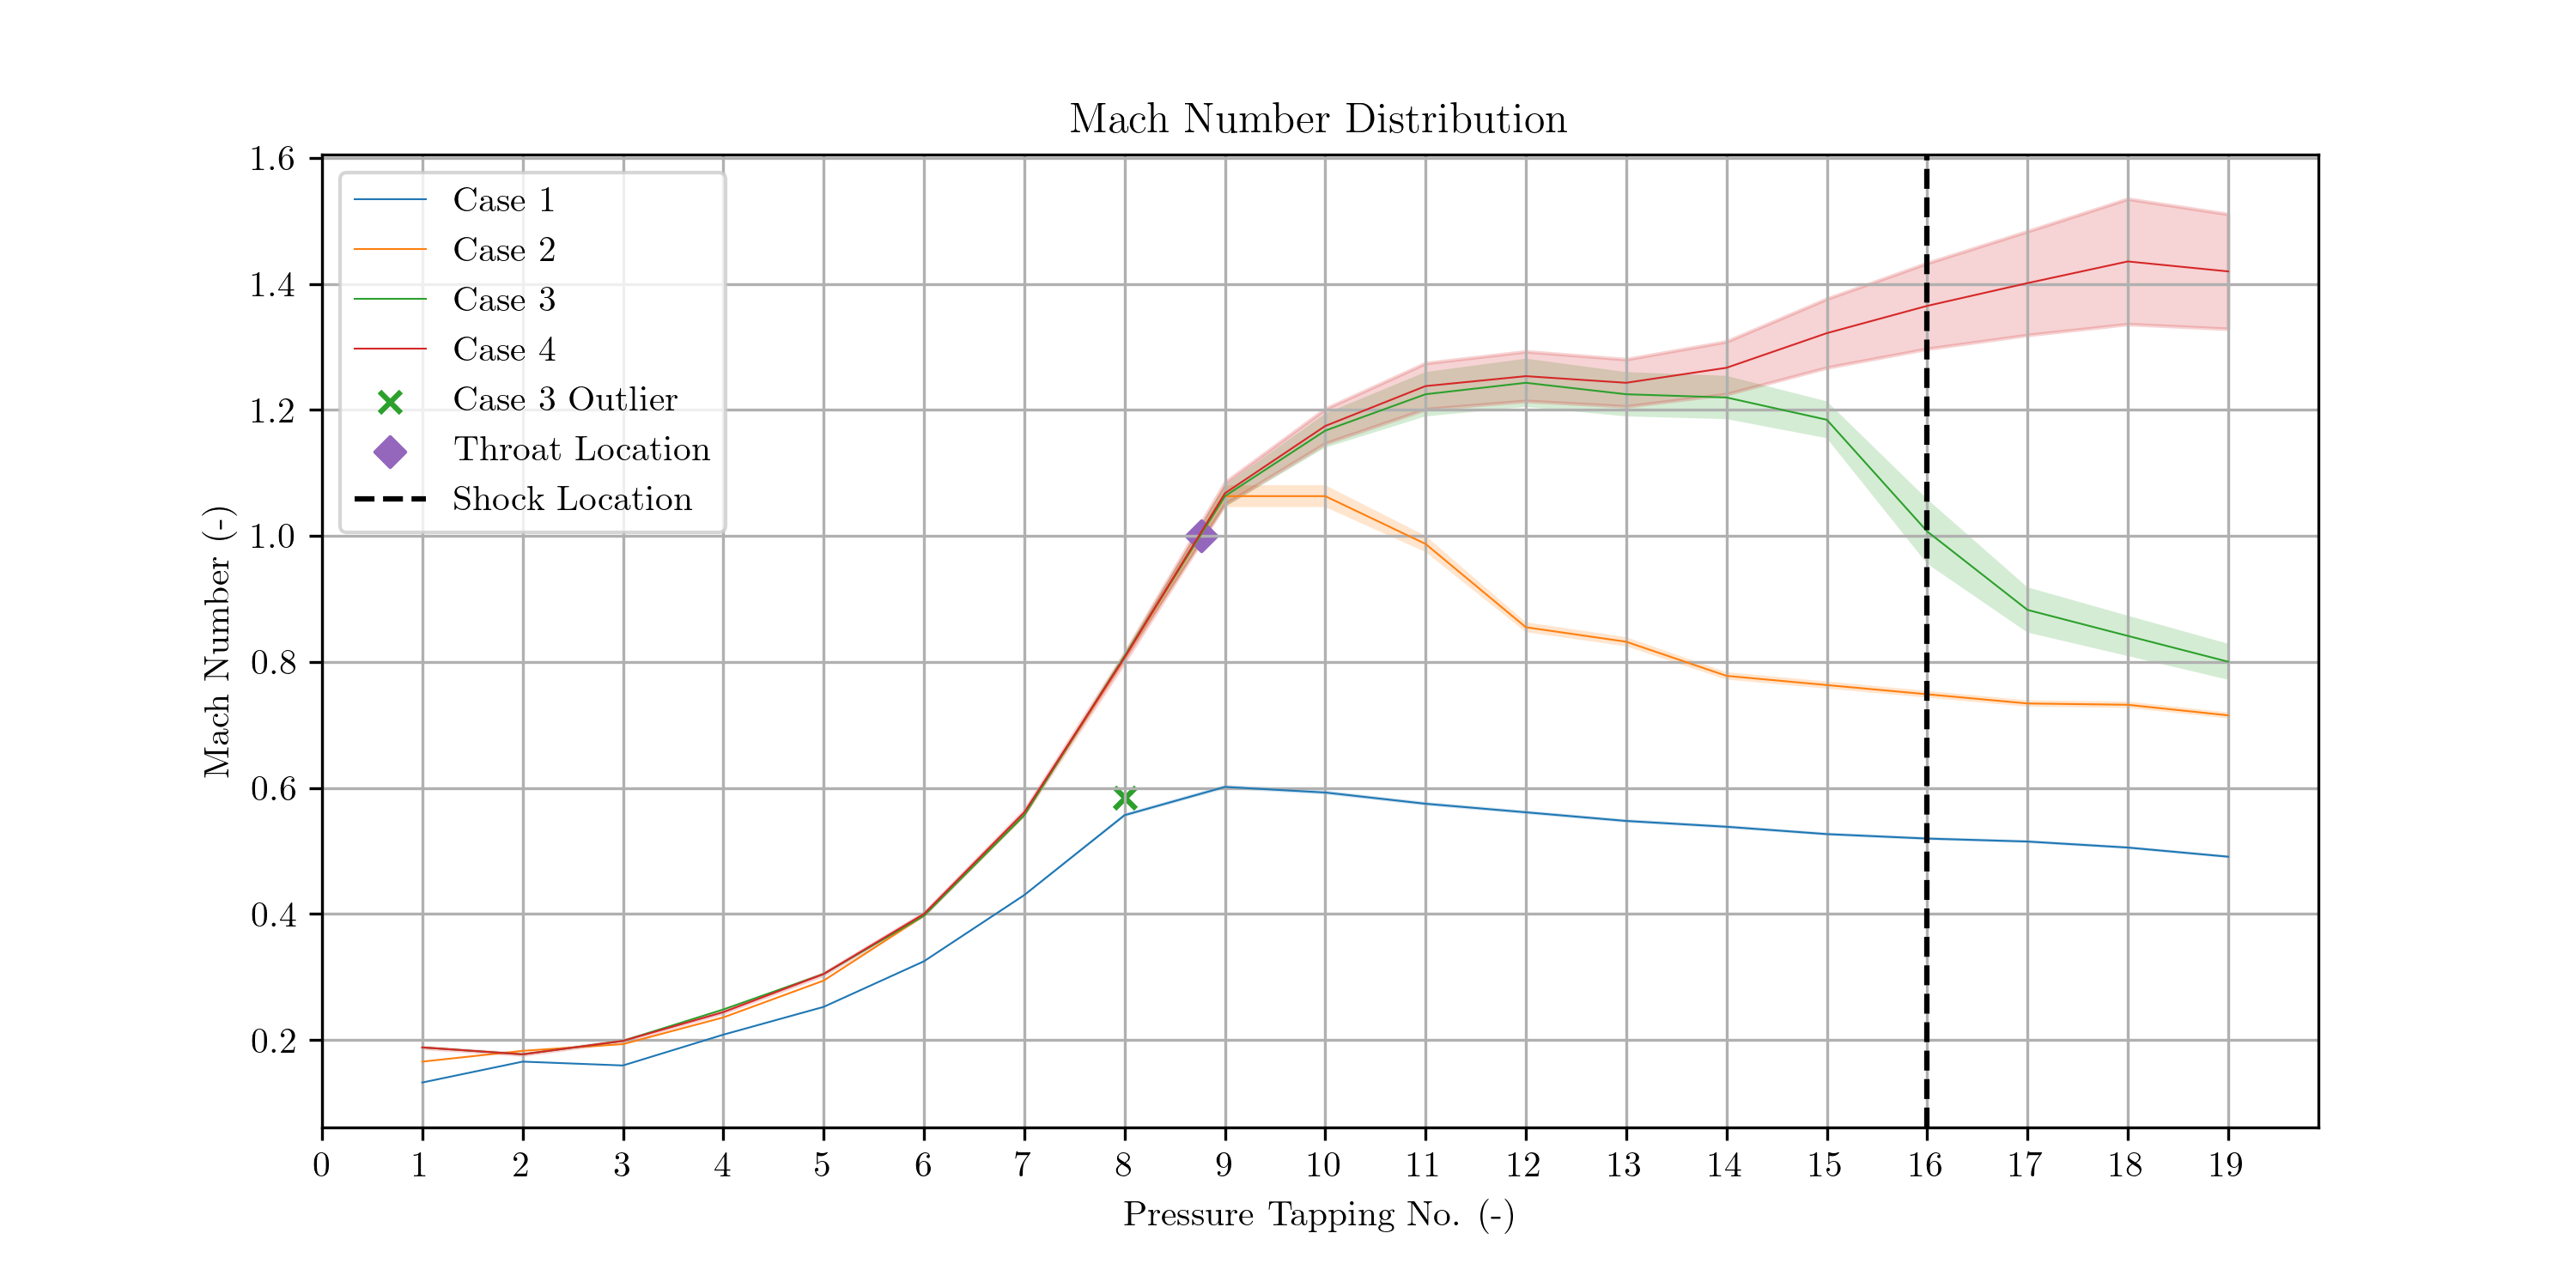
\includegraphics[width=0.98\textwidth]{../Supersonic_Nozzle/mach_number_distribution_corrected.png}
    \caption{Static pressure ratio distribution along the nozzle.}
    \label{fig:mach_distribution}
\end{figure}

\begin{figure}[H]
    \centering
    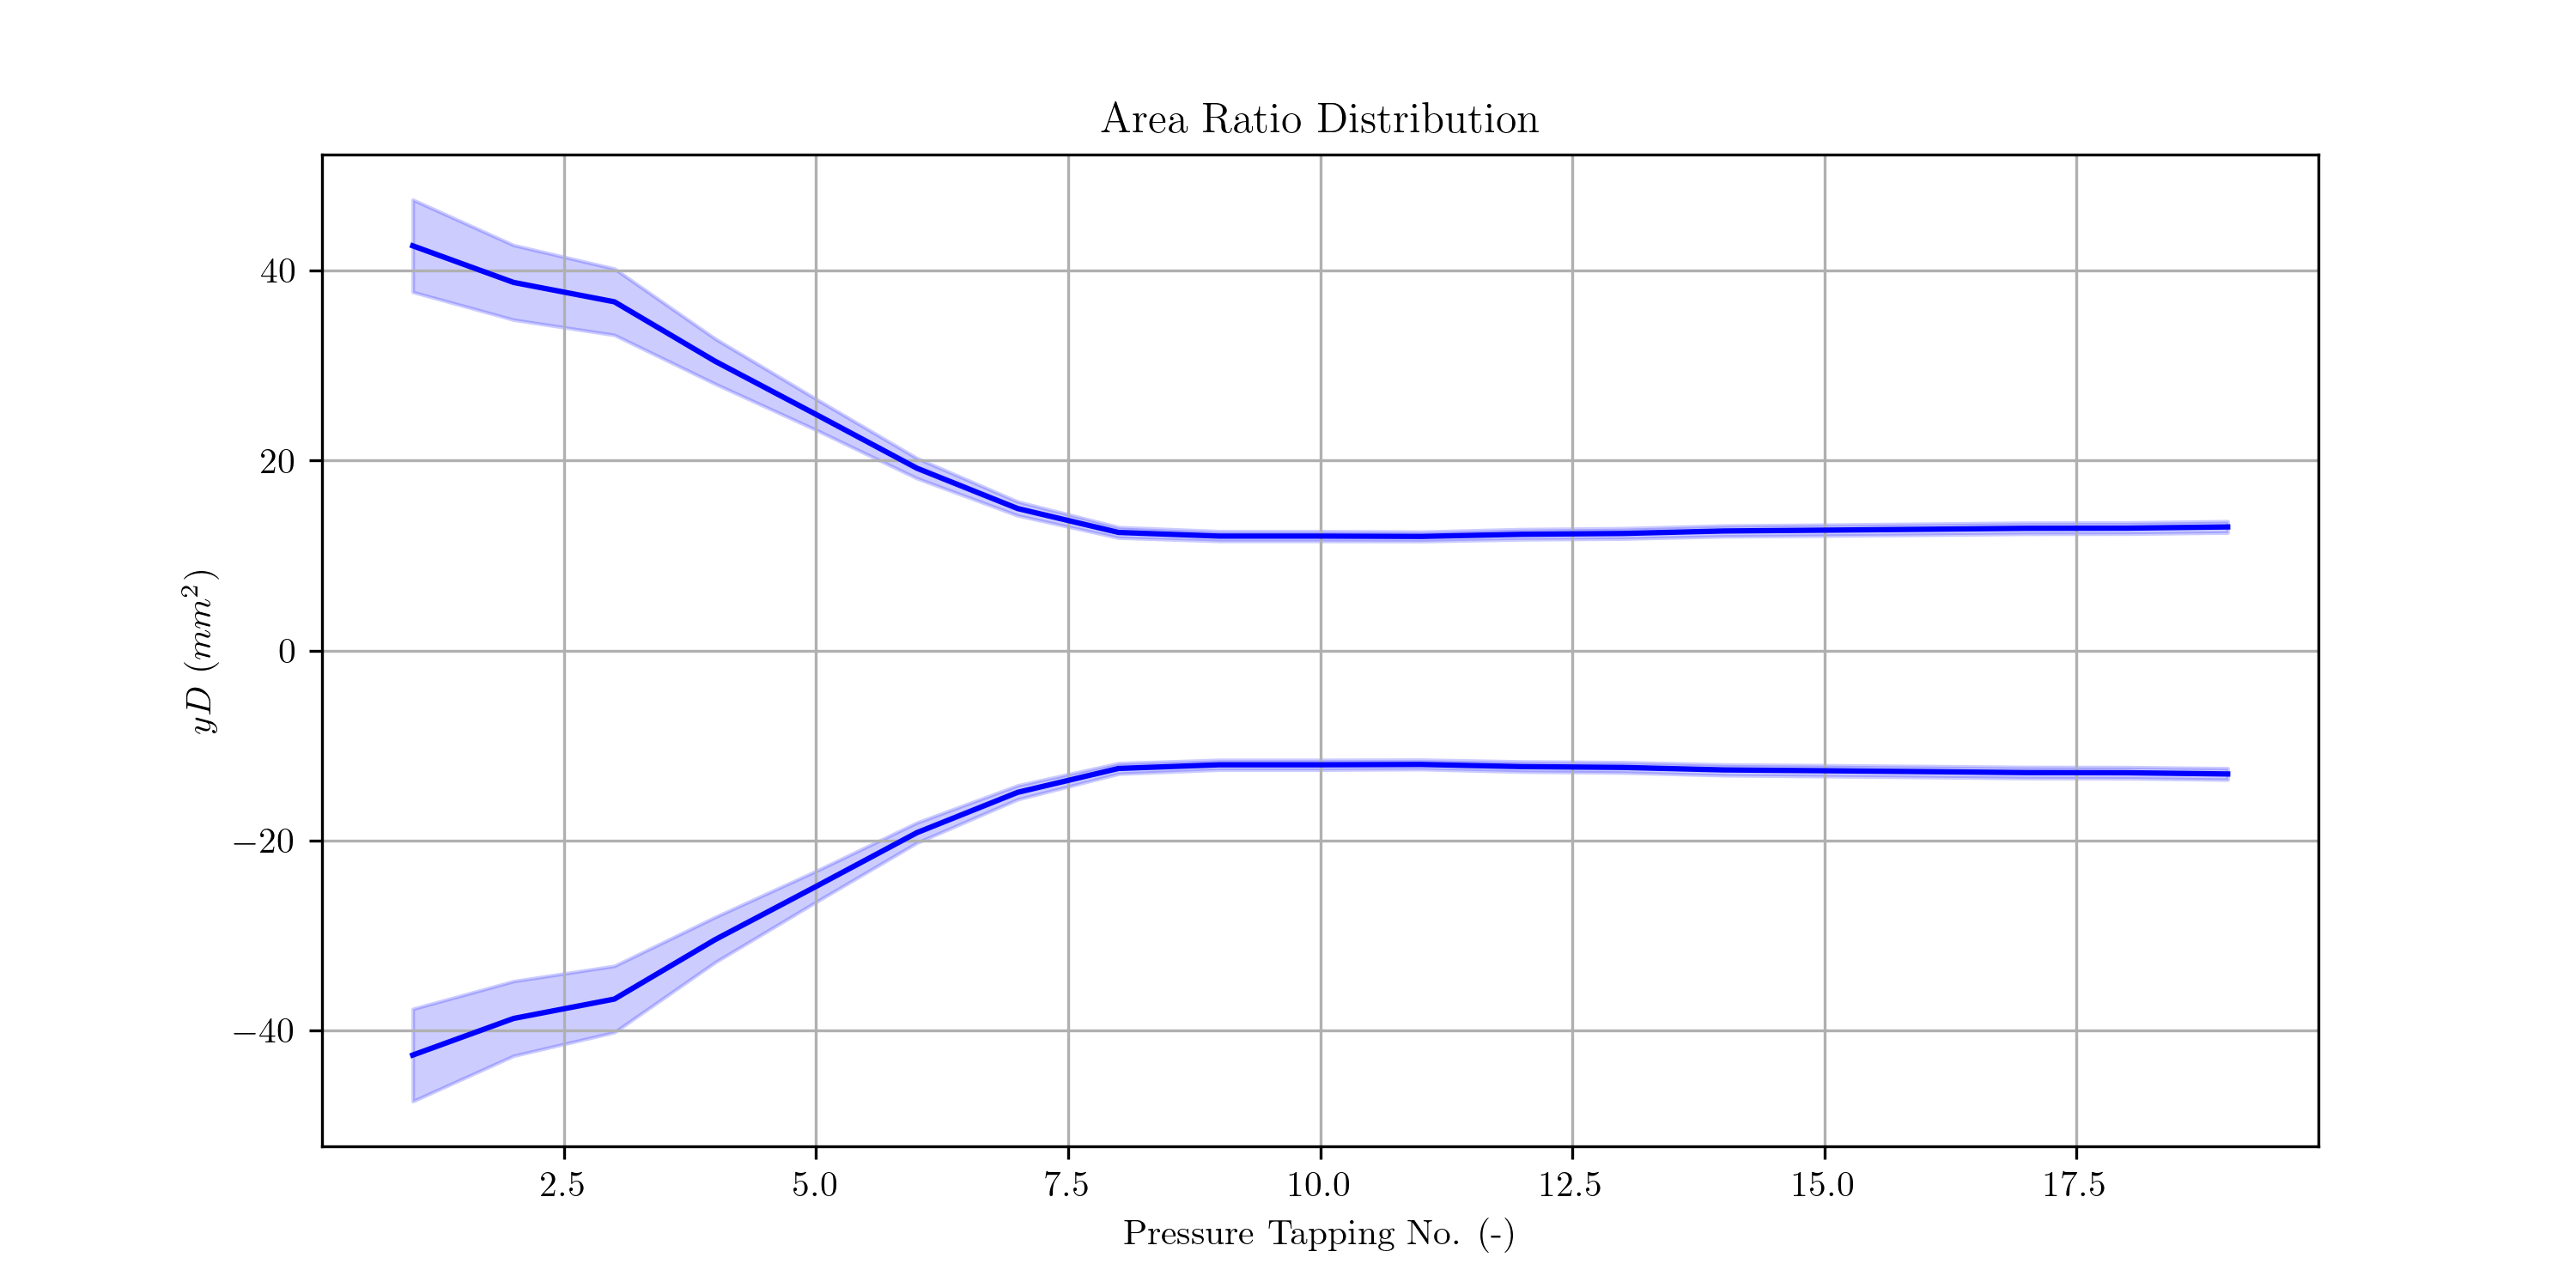
\includegraphics[width=0.98\textwidth]{../Supersonic_Nozzle/area_ratio_distribution.png}
    \caption{Reconstructed nozzle profile from throat area ratio.}
    \label{fig:area_distribution}
\end{figure}

\begin{figure}[H]
    \centering
    \begin{subfigure}[t]{0.48\textwidth}
        \centering
        \includegraphics[width=1\textwidth]{../Supersonic_Nozzle/shadowgraph_annotations/slide1.PNG}
        \caption{Shock wave in working section before sensors}

        \label{fig:figure6}
    \end{subfigure}
    ~
    \begin{subfigure}[t]{0.48\textwidth}
        \centering
        \includegraphics[width=1\textwidth]{../Supersonic_Nozzle/shadowgraph_annotations/slide2.PNG}
        \caption{Working state and bow shock of pitot probe}
        \label{fig:figure7}
    \end{subfigure}
    \caption{Schlieren images of the supersonic wind tunnel}
\end{figure}

\begin{figure}[H]
    \centering
    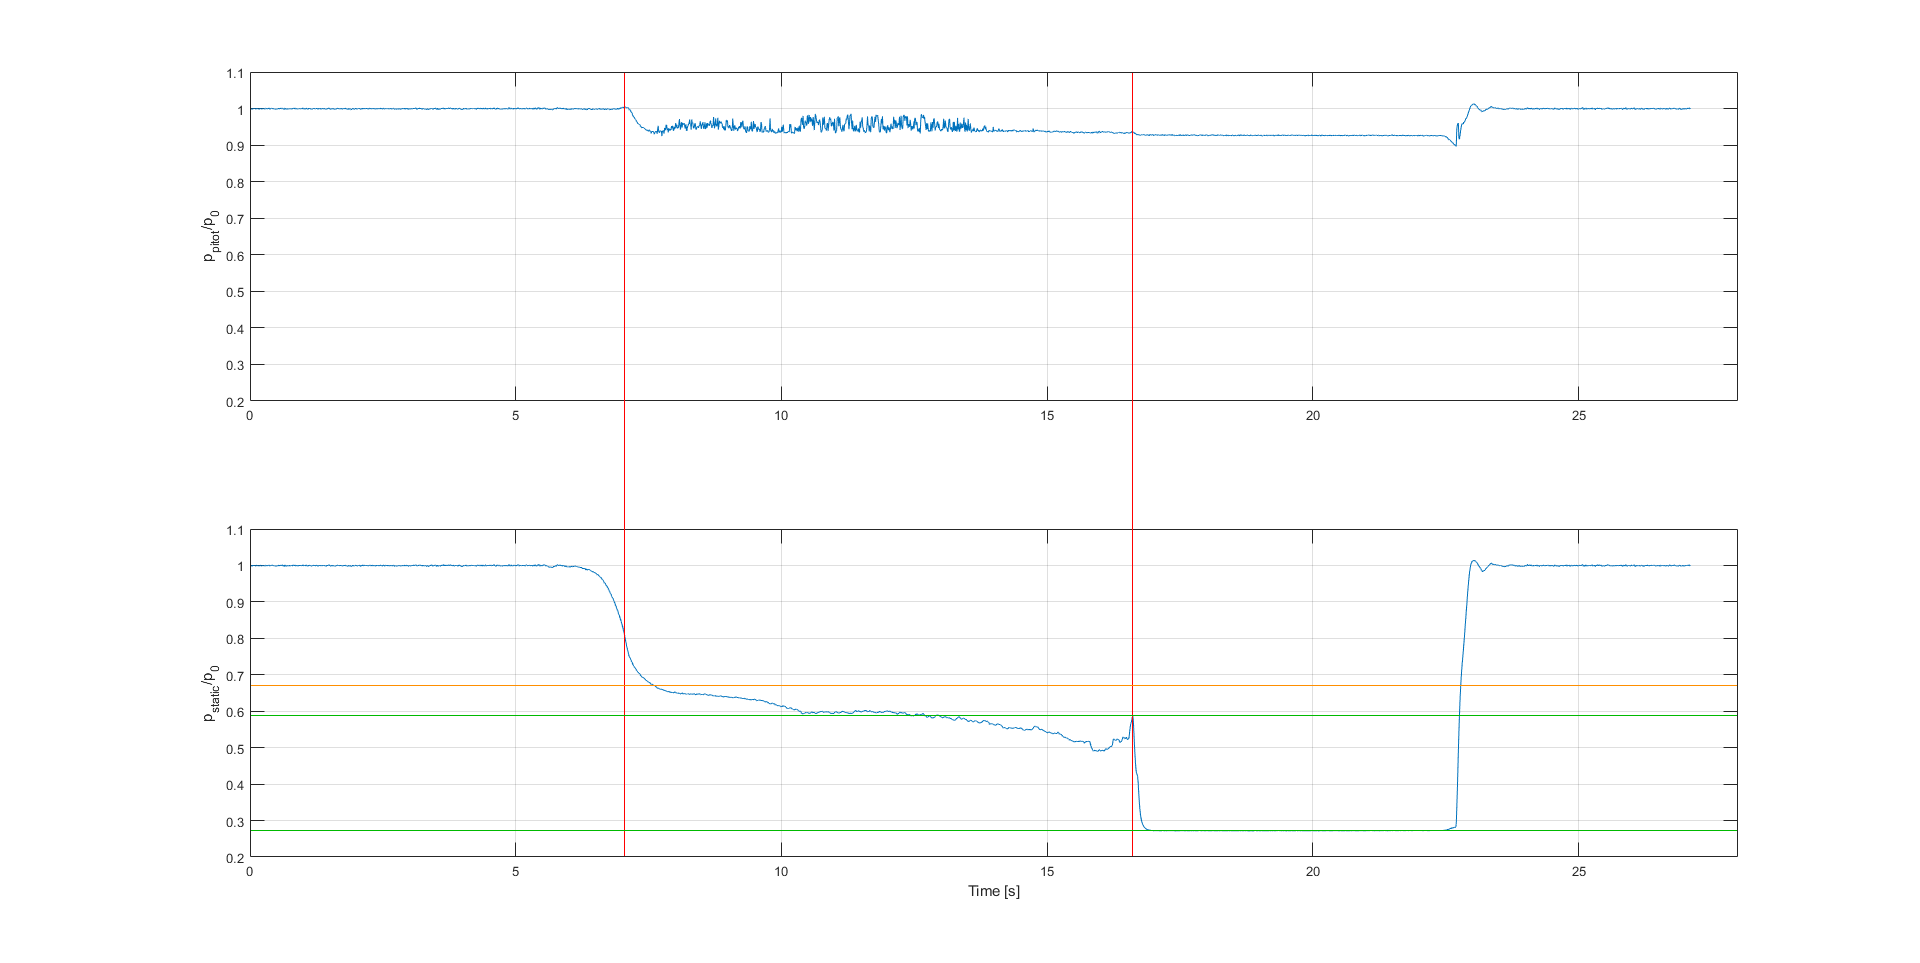
\includegraphics[width=1\textwidth]{../Supersonic_Nozzle/tunnel_pressures_annotated.png}
    \caption{Annotated readings of the pressure sensors over time during the experiment. Top graph shows the stagnation pressure ratio, and the bottom graph shows the static pressure ratio.}
    \label{fig:figure8}
\end{figure}

\section{Discussion}

\subsection{Part 1}

For run 3 of Part 1, determine the strength of the shock in the nozzle from its assumed location.
Indicate the expected (inviscid) pressure jump across the shock on your graph.

Using your measurement of mass flow in Part 1, calculate the cross-sectional areas of the throat and at
the nozzle exit for each run. In the case of Run 3 you need to first determine the expected stagnation
pressure drop through the shock wave before calculating the nozzle exit area. You should then attempt
to explain any differences you may find between the results of the different runs (note that the actual
cross-sectional area at the throat of the nozzle is approximately 24 mm2).

\subsection{Part 2}

Figure \ref{fig:figure6} shows the shock wave in the working section of the supersonic wind tunnel before the pressure sensors.
Shock waves of high density gradient are visible in the image from dark regions of the shadowgraph, where darker regions indicate stronger shock waves.
At the boundary layers at the top and bottom of the tunnel, the flow appears to travel through two shockwaves.
After the first shockwave the flow near the boundary layer is subsonic, but then must be accelerated again to supersonic speeds before the second, weaker shock.

Figure \ref{fig:figure8} shows the annotated readings of the pressure sensors over time during the experiment.
The green and red dots indicates the time at which the tunnel was switched on and off respectively.
It can be observed that before the first vertical red line, the static pressure decreases which corresponds to the subsonic flow accelerating.
At the first red line the stagnation pressure falls as the normal shock wave is formed upstream of the sensors by the, now supersonic, flow downstream of the throat.
The stagnation pressure readings then becomes very noisy as the shock wave moves further downstream due to complex shock boundary layer interactions.
The static pressure ratio slowly decreases over the next several seconds, indicating an acceleration in the flow, before quickly increasing again.
This may be due to the boundary layer growing and then shrinking rapidly, acting similarly to a convergent divergent nozzle, as the shock wave moves closer to the sensors.
The second vertical red line shows where the shock wave passes the sensors and static pressure drops significantly.

After the shock has passed, the bottom green line shows a static pressure ratio of around $p/p_0 = 0.275$. This corresponds to a Mach number of 1.49, which is very close to the set operating point of Mach 1.5.
From the databook, at Mach 1.5 the pressure ratio accross the shock should be $p_s/p = 2.4583$.
Multiplying this by the measured static pressure ratio after the shock passes, gives us the theoetical static pressure ratio before the shock passed, which is $p_s/p_0 = 0.275 \times 2.4583 = 0.676$, and is shown by the orange horizontal line.
The actual pressure ratio behind the shock, given by the pressure at the time before the shock passes the sensors, is shown by the top green line at $p_s/p_0 = 0.59$.
This shows that the actual pressure drop accross the shock is less than the theoretical value for Mach 1.5.
It seems that the flow after the shock is at a higher Mach number than expected due to the boundary layer effects.

The pitot probe should show an increase in stagnation pressure after the shock wave passes, however it can be observed that this remains nearly unchanged.
The expected stagnation pressure ratio downstream of the shock can be calculated from Equation 8 for Mach 1.5 and is found to be 0.9298. This very close to the value seen, however after the shock passes the stagnation pressure ratio should increase back to 1.0.
It can be observed from figure \ref{fig:figure7} that a bow shock forms in front of the pitot probe and so the shock effectively never passes the probe, which explains why the stagnant pressure ratio does not increase back up to 1.0.

Compare the two experiments. Are there any findings that can be related from one experiment to the other?
What have you learned about the interaction of a shock wave with a boundary layer?

\section{Conclusion}
% Comment on the validity of one-dimensional theory in nozzle flows. When can it be expected to provide what quality of predictions?
% What are the effects of viscosity in both experiments? Which experiment is more severely affected and why?

Comment on the validity of one-dimensional theory in nozzle flows. When can it be expected to
provide what quality of predictions?
What are the effects of viscosity in both experiments? Which experiment is more severely affected
and why?

\newpage

\section{Appendix}

The following equations are used to calculate uncertainty in area ratio.

\begin{equation}
    u(A) = u(A^*) + u\left( \frac{A}{A^*} \right) = u(A^*) + u(M) \frac{d}{dM}\left( \frac{A}{A^*} \right)
\end{equation}

\begin{equation}
    \frac{d}{dM}\left( \frac{A}{A^*} \right) = \frac{2 \left(\frac{2 \left(M^{2} \left(\frac{\gamma}{2} - \frac{1}{2}\right) + 1\right)}{\gamma + 1}\right)^{\frac{\gamma + 1}{2 \gamma - 2}} \left(\frac{\gamma}{2} - \frac{1}{2}\right) \left(\gamma + 1\right)}{\left(2 \gamma - 2\right) \left(M^{2} \left(\frac{\gamma}{2} - \frac{1}{2}\right) + 1\right)} - \frac{\left(\frac{2 \left(M^{2} \left(\frac{\gamma}{2} - \frac{1}{2}\right) + 1\right)}{\gamma + 1}\right)^{\frac{\gamma + 1}{2 \gamma - 2}}}{M^{2}}
    \label{eqn:dA_dM}
\end{equation}

The following equations are used to correct for the drop in stagnation pressure accross the shock wave in Case 3.

\begin{equation}
    \frac{p_{0s}}{p_0} = \left( \frac{\frac{\gamma+1}{2}M^2}{1 + \frac{\gamma-1}{2}M^2}\right) ^ \frac{\gamma}{\gamma-1} \left( \frac{2\gamma}{\gamma+1} M^2 - \frac{\gamma-1}{\gamma+1}\right) ^ \frac{1}{1 - \gamma}
\end{equation}

\begin{equation}
    u\left( \frac{p_{0s}}{p_0} \right) = u(M) \frac{d}{dM}\left( \frac{p_{0s}}{p_0} \right)
\end{equation}

\begin{equation}
    \begin{aligned}[b]
    & \frac{d}{dM}\left( \frac{p_{0s}}{p_0} \right) = - \frac{4 M \gamma \left(\frac{M^{2} \left(\frac{\gamma}{2} + \frac{1}{2}\right)}{M^{2} \left(\frac{\gamma}{2} - \frac{1}{2}\right) + 1}\right)^{\frac{\gamma}{\gamma - 1}} \left(\frac{2 M^{2} \gamma}{\gamma + 1} - \frac{\gamma - 1}{\gamma + 1}\right)^{- \frac{1}{\gamma - 1}}}{\left(\gamma - 1\right) \left(\gamma + 1\right) \left(\frac{2 M^{2} \gamma}{\gamma + 1} - \frac{\gamma - 1}{\gamma + 1}\right)} \\
    & + \frac{\gamma \left(\frac{M^{2} \left(\frac{\gamma}{2} + \frac{1}{2}\right)}{M^{2} \left(\frac{\gamma}{2} - \frac{1}{2}\right) + 1}\right)^{\frac{\gamma}{\gamma - 1}} \left(M^{2} \left(\frac{\gamma}{2} - \frac{1}{2}\right) + 1\right) \left(\frac{2 M^{2} \gamma}{\gamma + 1} - \frac{\gamma - 1}{\gamma + 1}\right)^{- \frac{1}{\gamma - 1}} \left(- \frac{2 M^{3} \left(\frac{\gamma}{2} - \frac{1}{2}\right) \left(\frac{\gamma}{2} + \frac{1}{2}\right)}{\left(M^{2} \left(\frac{\gamma}{2} - \frac{1}{2}\right) + 1\right)^{2}} + \frac{2 M \left(\frac{\gamma}{2} + \frac{1}{2}\right)}{M^{2} \left(\frac{\gamma}{2} - \frac{1}{2}\right) + 1}\right)}{M^{2} \left(\frac{\gamma}{2} + \frac{1}{2}\right) \left(\gamma - 1\right)}
    \end{aligned}
    \label{eqn:dp0sr_dm}
\end{equation}
\footnotetext{Equations for derivatives \ref{eqn:dA_dM} and \ref{eqn:dp0sr_dm} were generated using SymPy from databook equations \cite{data_book}.}


\begin{figure}[H]
    \centering
    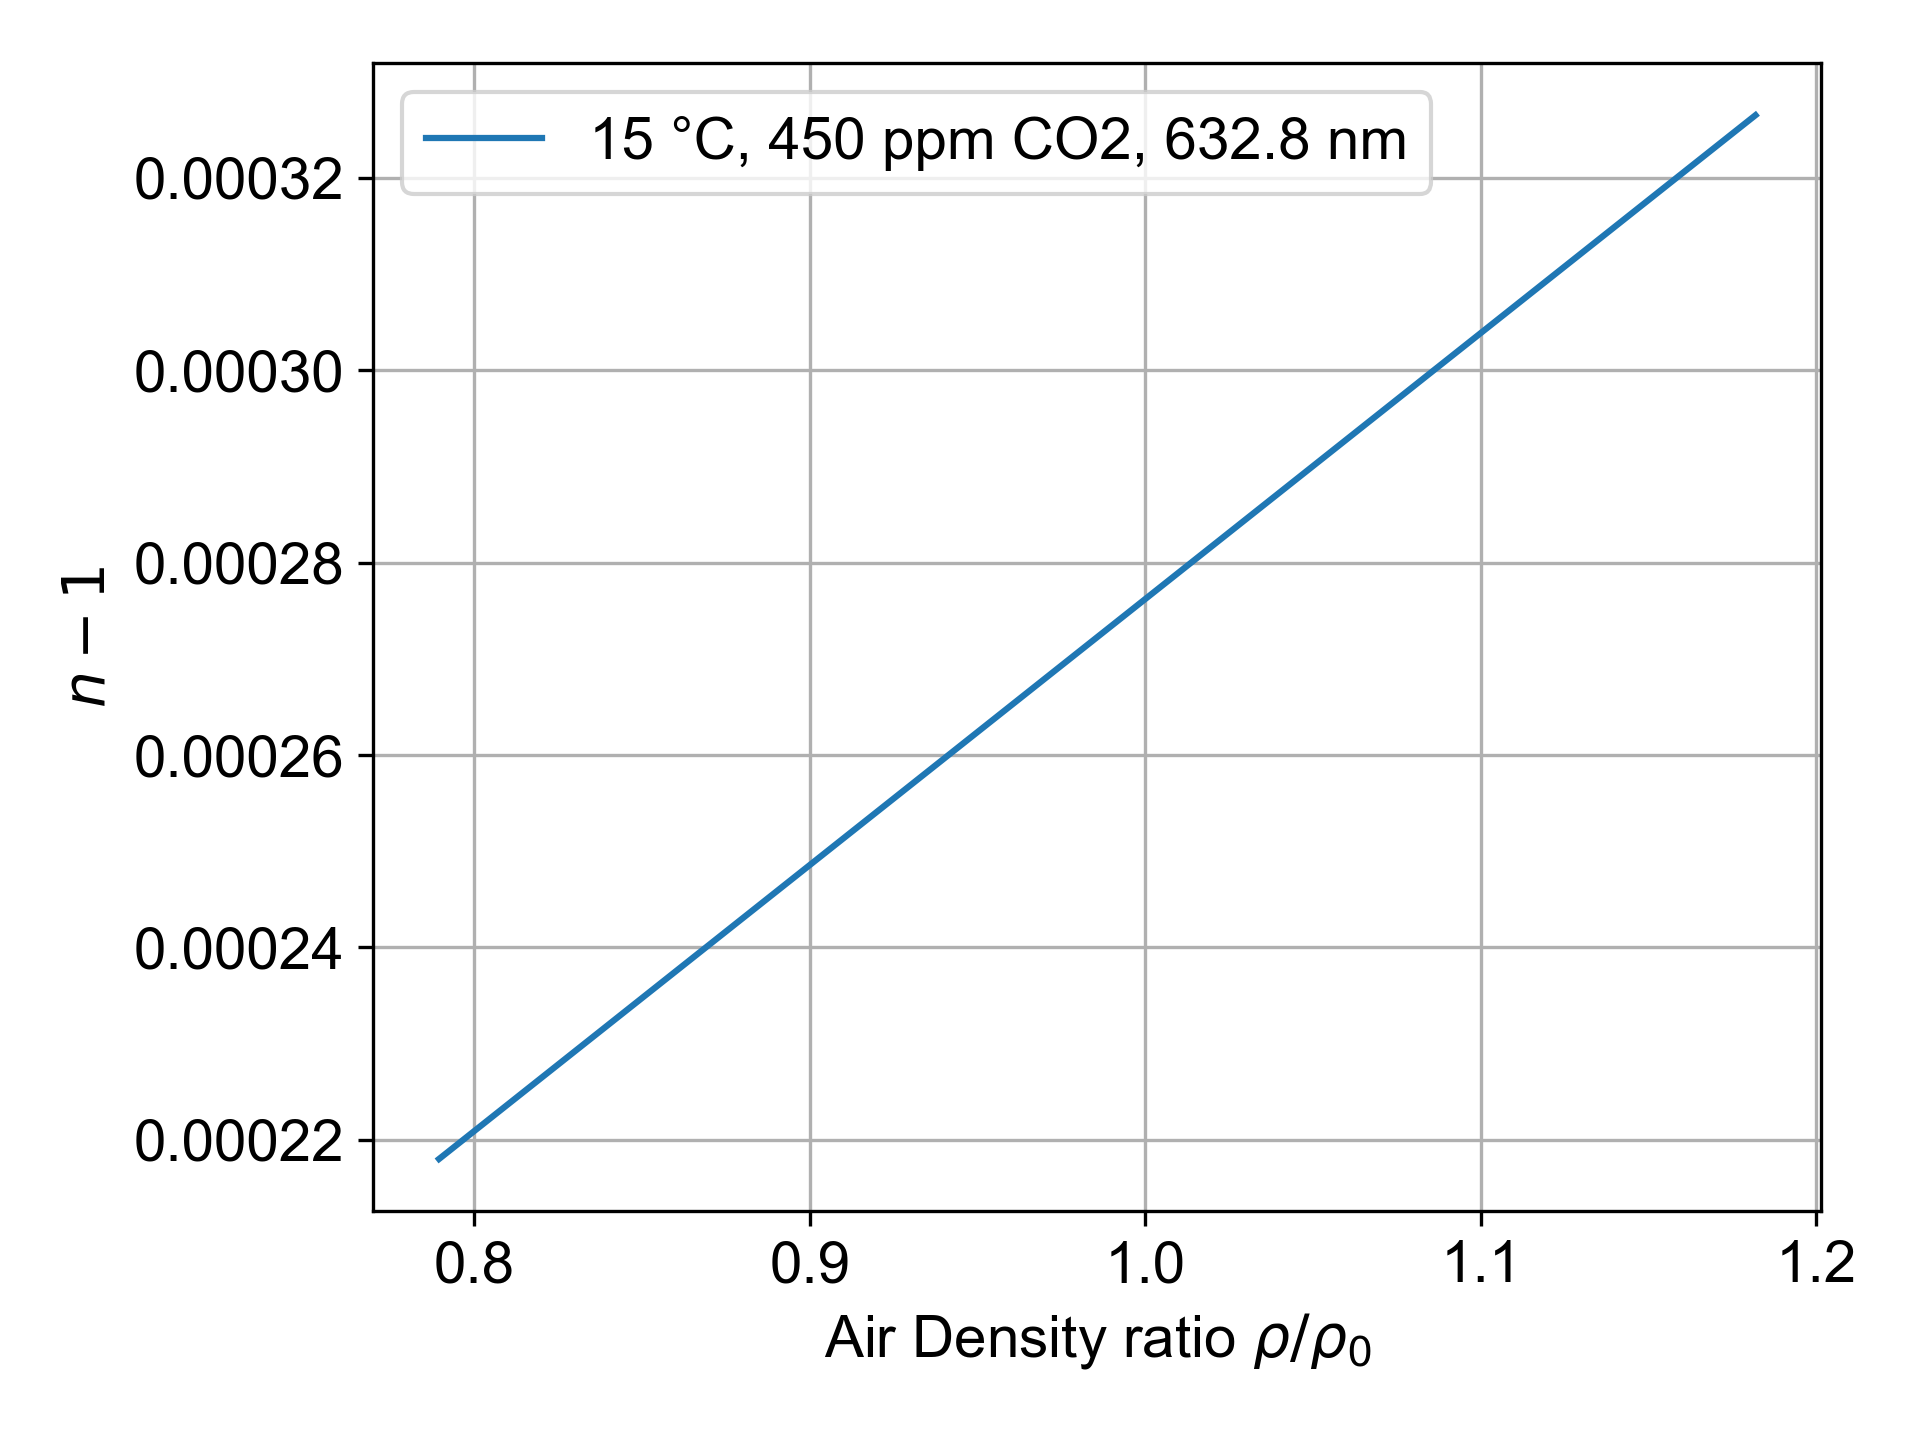
\includegraphics[width=0.6\textwidth]{dry_air_15_rho_vs_n.png}
    \caption{Refractive index $n-1$ against density ratio $\rho/\rho_0$ for relative humidity $\phi = 50\%$, 450 ppm $ \text{CO}_2 $, wavelength $\lambda = 632.8$ nm. Figure produced from modified code \cite{refractiveindex_info} using equations by Ciddor, 1996 \cite{Ciddor:96}.}
    \label{fig:refractive_index_vs_density}
\end{figure}

\begin{figure}[H]
    \centering
    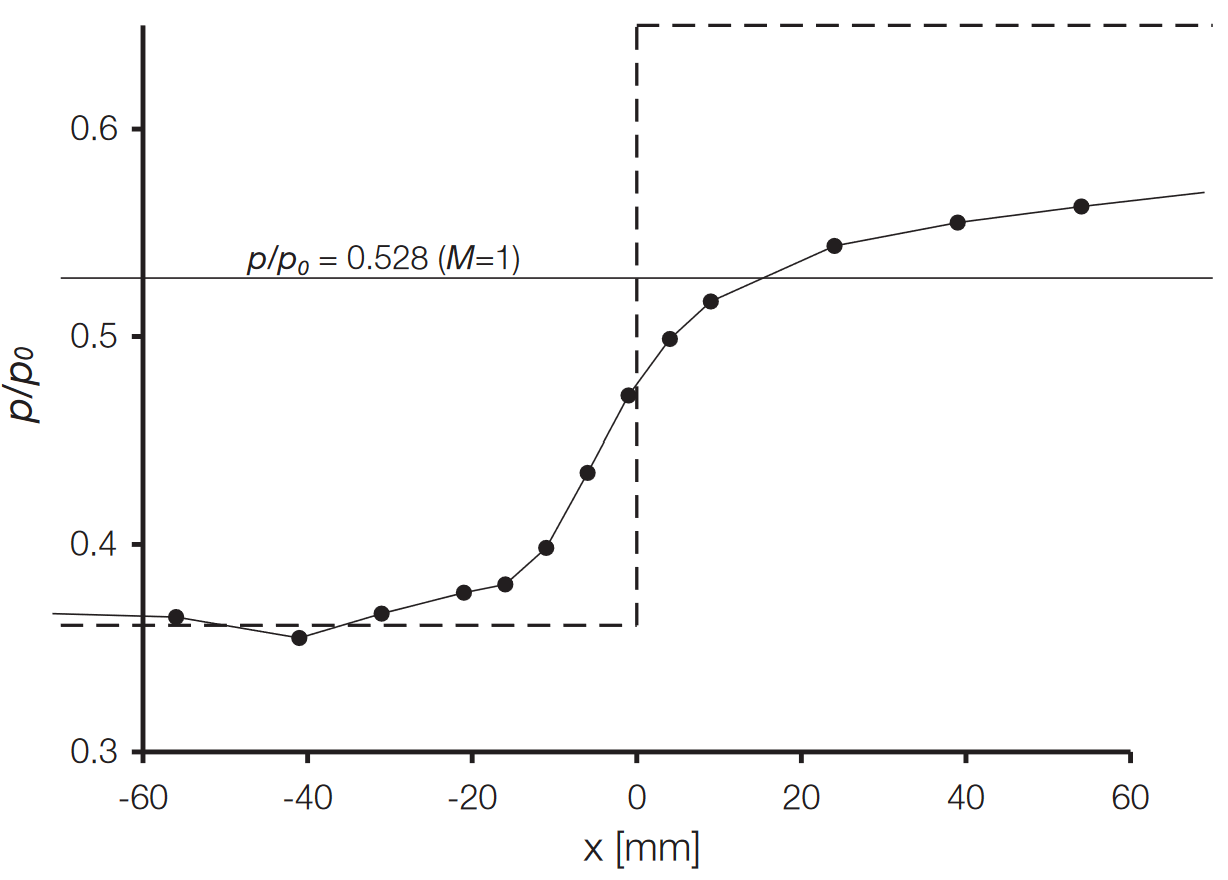
\includegraphics[width=0.6\textwidth]{SBLI_pressure_smearing.png}
    \caption{Static wall pressure distribution at the shock boundary layer interaction \cite{babinsky_delery:2011}.}
    \label{fig:SBLI_pressure_smearing}
\end{figure}

\begin{figure}[H]
    \centering
    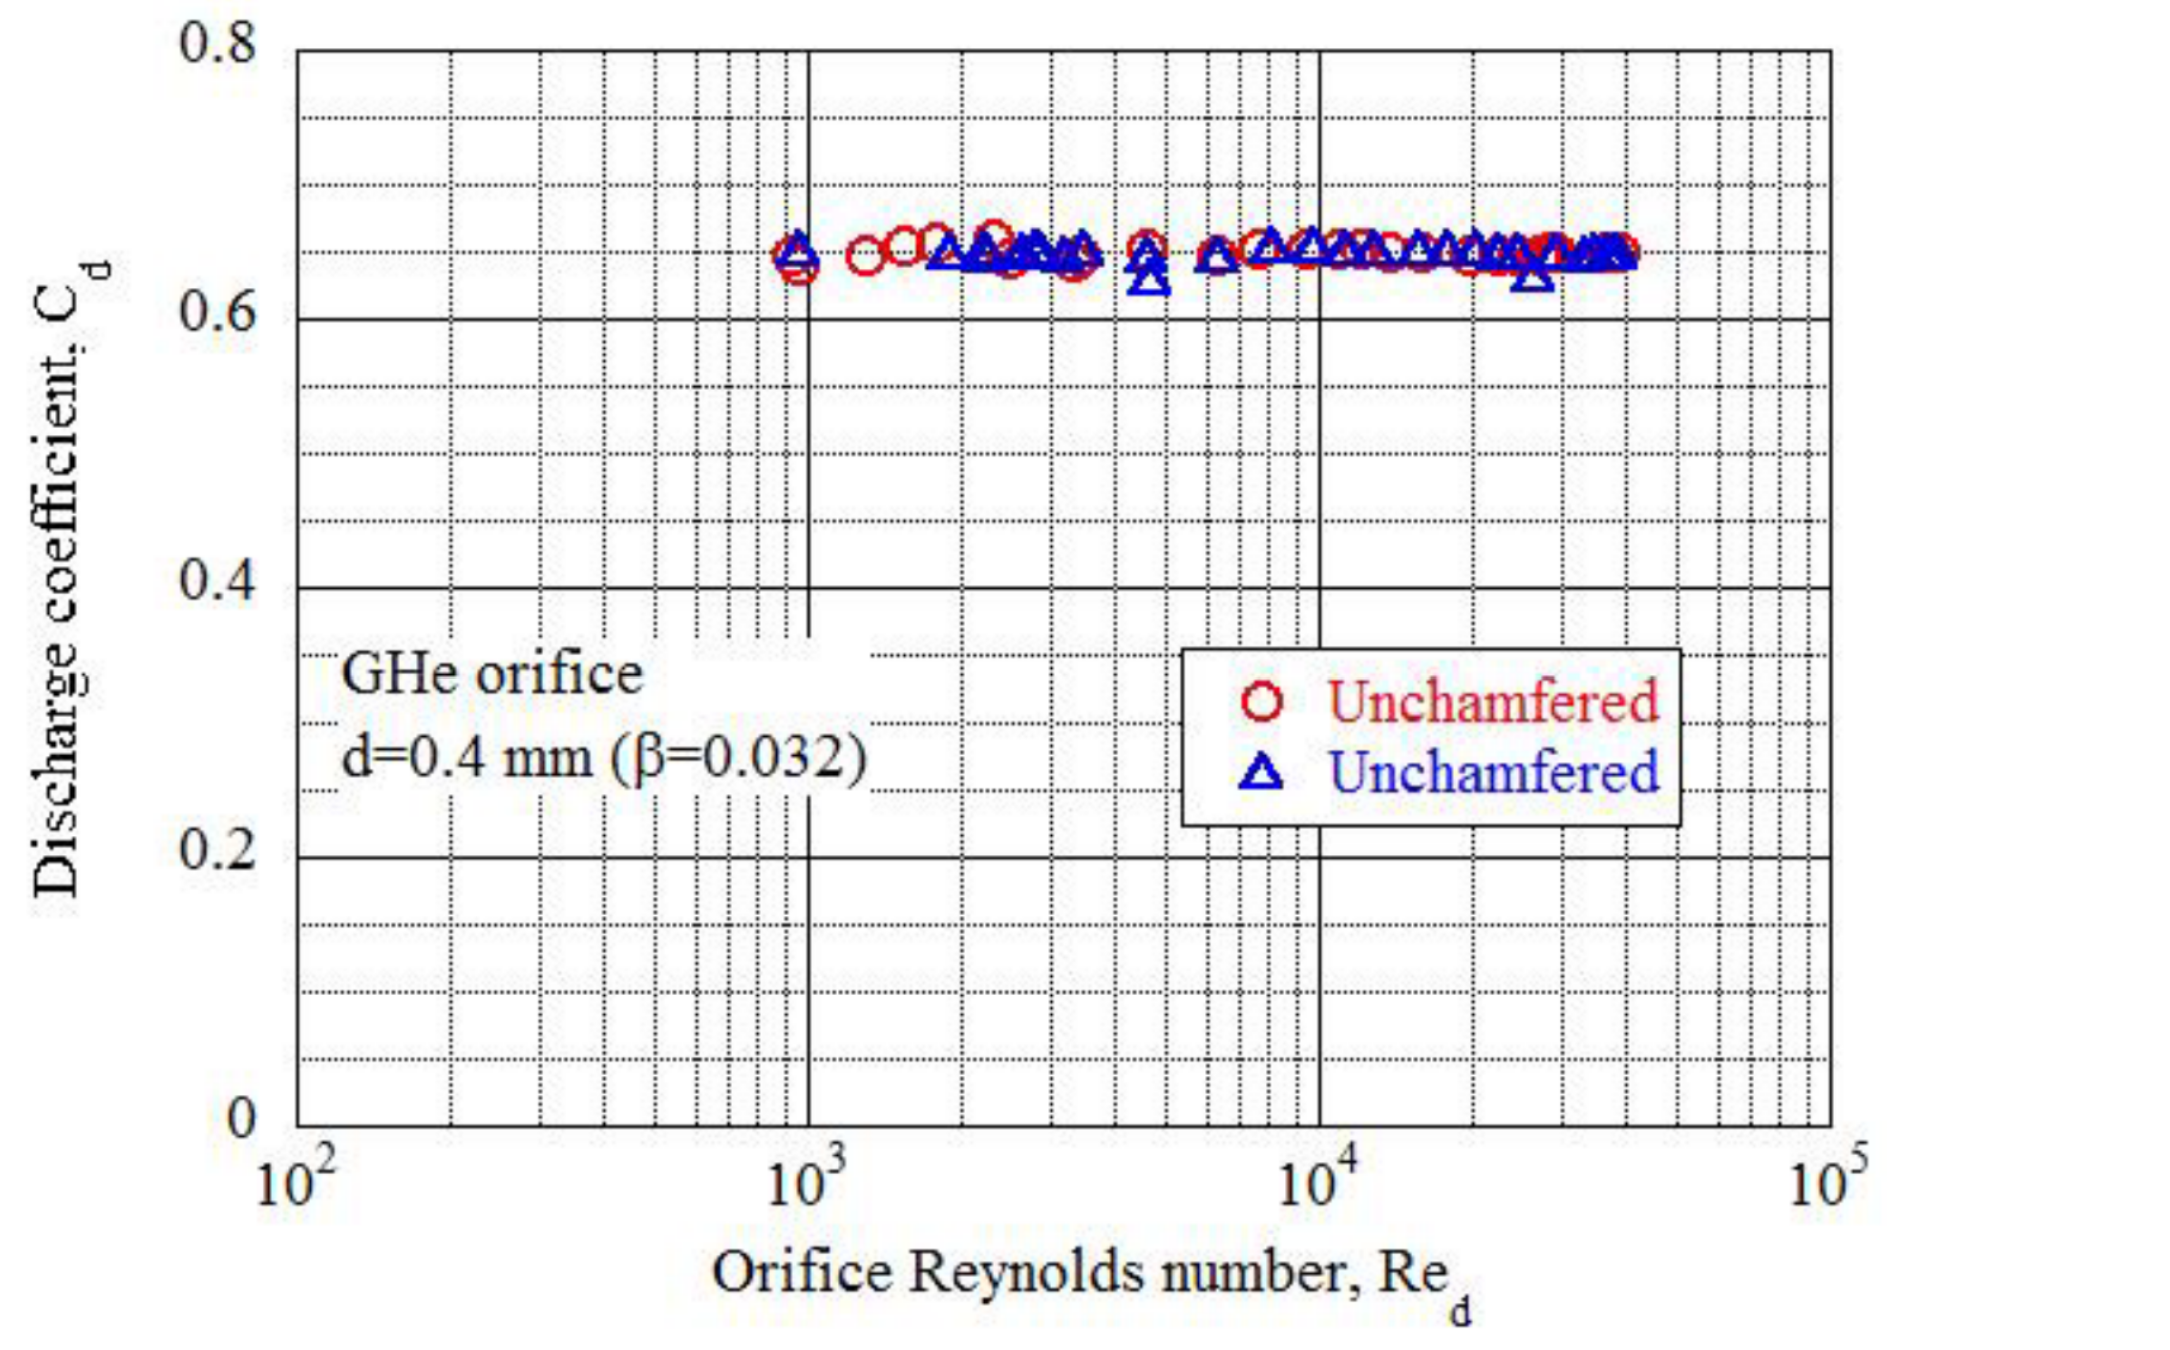
\includegraphics[width=0.6\textwidth]{Graham_K_Webster_const_Cd_Re.png}
    \caption{Constant discharge coefficient for high Reynolds numbers \cite{Graham_K_Webster:2019}.}
    \label{fig:const_Cd_Re}
\end{figure}

\bibliographystyle{plain}
\bibliography{refs}

\end{document}